\protect\hypertarget{titlepage.xhtml}{}{}

\protect\hypertarget{index_split_000.html}{}{}

NO. 6 \textbar{} Atsuko Asano

\protect\hypertarget{index_split_001_split_002.html}{}{}

\hypertarget{index_split_001_split_002.htmlux5cux23calibre_pb_0}{%
\subsection{Volume
4}\label{index_split_001_split_002.htmlux5cux23calibre_pb_0}}

\emph{We're coming back alive. Don't forget that. .}

\hypertarget{index_split_001_split_002.htmlux5cux23calibre_pb_1}{}

\hypertarget{index_split_001_split_002.htmlux5cux23calibre_pb_0}{}

\hypertarget{index_split_001_split_002.htmlux5cux23calibre_toc_2}{%
\subsection{CHAPTER
1}\label{index_split_001_split_002.htmlux5cux23calibre_toc_2}}

\subsubsection{Curtain Up}

\emph{Howl, howl, howl! O, you are men of stones!}

\emph{Had I your tongues and eyes, I'd use them so}

\emph{That heaven's vault should crack! She's gone fore ever.}

\emph{- King Lear Act V Scene III}

Beyond the gate was a world of darkness.

It was freezing. The man shivered, and flipped the collar of his jacket
up. His coat was woven of the finest cashmere, and it was lightweight
and warm. It was also equipped with an automatic sensor that registered
the temperature of the body and outside air to adjust the temperature
inside the coat accordingly. The sensor itself was smaller, lighter, and
slimmer than a postage stamp.~

He could feel the biting coldness of the air on his partially-exposed
face, but the rest of his body was enveloped comfortably in the warmth
of his coat. So when the man shivered, it was not because of the cold.

It was the darkness. It was too dark.

No. 6, where the man lived, was a city of light. It sparkled and brimmed
with it, regardless of whether it was day or night. Light wasn't the
only thing he had access to freely: thanks to leaps in biotechnology, a
steady supply of food was always available, independent of seasonal or
weather conditions, and he had access to any manner of foodstuffs. It
was the same with energy supply. As long as they were inside the city,
people were able to lead an abundant, secure and hygienic life. Apart
from them, there were five other city-states in the world, but no other
place had an environment as perfect as theirs. This was the reason
behind No. 6's second name of the Holy City.

The man held an important position in the governing body of the Holy
City. Inside the Central Administration Bureau, he held what was
equivalent to the third most powerful spot. He was an elite of the
elites. His son, who was turning three this year, had also scored
highest in intelligence in the past Children's Examinations. The man was
already receiving childrearing instruction through a Special Curriculum.
If no problems arose ― no problems would arise, naturally, because in no
way would anything unpredictable happen inside the Holy City ― then his
son, as an elite as well, would be able to acquire a life which lacked
nothing. It was promised to him.

The man couldn't stop shivering. How dark it was. How foreboding it was.
He had no idea that nighttime could bring such fathomless darkness. He
had had no idea, until he had stepped into this West Block.

What the hell is he doing?

The man who was supposed to be there to fetch him, wasn't. He was
usually waiting for him in the cover of darkness, but tonight, there was
no sign of him at all.

Has something happened?

Maybe something has come up.

If so... then it isn't very good.

The man exhaled in the darkness.

It was best not to dawdle here any longer. He must pass back through the
gates, and return to the Holy City. He must.

His reason commanded him to return, to turn on his heel, and go back
into comfort and light. But the man could not move.

Just a little longer. I'll wait for five more minutes.

It was a lingering attachment. It was his attachment for the few hours
of pleasure and decadence that he was about to enjoy. This attachment,
for the few hours he spent fooling around with women in the West Block,
weighed his feet down and prevented him from walking away. How enticing
it was to spend the hours in a drunken stupor, in the company of women
with hair and eyes in every colour. It was almost a year now since he
had first been irresistibly drawn into this enticement. There was no way
out of it.

The City's management was getting stricter. General citizens were
restricted, naturally; but even the upper echelons, which had had
considerable freedom, were being imposed with limitations. Travel
between the city and the West Block was one of the things which limits
had been placed upon.

All travel between other Blocks were prohibited unless with a clear
reason and an application to do so.

When the man had seen that section of the city's notice, he remembered
giving a small sigh. The Central Administration Bureau was a department
that singularly managed all of the city's information. All personal
files of the citizens were naturally gathered here as well. Each
citizen's name, sex, birth date, family structure, intelligence index,
physical characteristics, physical measurements, history of illness,
curriculum vitae, were all contained here. The daily actions of each and
every individual were recorded without fail and internalized as data by
the Central Administration Bureau, through the numerous surveillance
cameras and sensors placed throughout the city, as well as the
data-collection chips embedded in their ID cards. This system was
already well-established.

Thorough management and centralization of data ― and whether for better
or for worse, this man was near the heart of the system. He used his
position to his advantage to overwrite his personal records numerous
times. He had rewritten his file to say he had never entered the West
Block. He had destroyed his records.

It was a crime, he was well aware. He was nervous of what would happen
to him if this was exposed, and at the same time, he was confident that
he would never be found out. He drowned himself in euphoric ecstasy. At
the same time, he wanted to protect his secure life and cowered at its
destruction. And underneath was the confident reassurance that he was an
irreplaceable member of the elite core, and that he would not be
persecuted so easily. Many emotions jostled inside the man.

But in the end, he had given into his desires and passed through the
gates again tonight.

He's late, a little too late....

The man chewed his lip lightly.

I should probably give up for tonight.

Nothing was more dangerous than standing still like this for a prolonged
time, wrapped in the darkness of the West Block. As the man turned to go
back the way he had come, a low voice called his name.

"Fura-sama." That was the man's name. The low voice carried over to him
in the darkness. "I apologize for keeping you waiting."

Fura furrowed his brow, and hunched his shoulders slightly.

"Is it you, Rikiga?"

"Yes. I've come to fetch you."

"You're late."

"I'm terribly sorry. There was a slight delay."

"Delay? What happened?"

He could sense the darkness shift slightly as Rikiga shook his head.

"Nothing to worry yourself about. No trouble for you in the slightest
sense, Fura-sama... actually ― ah ― you could say I was delayed for the
purpose of your further enjoyment―"

"Which is to say?"

He could hear a vulgar laugh.

"It's taken me a bit of time to prepare a woman to your liking." The
vulgar laugh continued, and the darkness coiled slimily. "But rest
assured, it shall more than make up for the time I've kept you waiting.
I'm most certain you'll be satisfied."

"Is she that good?"

"Exquisite specimen."

He swallowed. If he could, he would have raised his own vulgar chuckle
like Rikiga, but he restrained himself.

His position was like the heavens in relation to Rikiga as the lowly
earth. a resident of the West Block. He could not bring himself down to
that level.

For Fura, although the West Block was place that provided him with lewd
and luscious pleasures, those who lived there ― Rikiga, or the women ―
were not the same humans as he. He saw them as insects, perhaps. No,
that was too harsh ― they were rather close to cattle. Humans and
cattle, the dominator and dominated. No. 6's surrounding regions existed
to serve the city ― that was what he had been taught since childhood.

"―Shall we go, then?" Rikiga began to walk. Silently, he followed
behind.

The outdated gasoline automobile was uncomfortable to ride, and bumped
and jerked ever so often. The road itself was full of potholes. Once in
a while, the car teetered dangerously. When Fura had first begun
frequenting the West Block, he had more than once raised his voice in
complaint, but now, he thought nothing of it. As one who was used to the
immaculately-paved roads of No. 6 and hybrid cars fully equipped with
shock-absorption, the sudden bumps and sways were new and refreshing.
And more than anything, it tickled his heart with the anticipation for
things to come.

"So?"

Fura leaned forward in the back seat and questioned him.

"What kind of girl is she?"

"I daresay she's a perfect match for your tastes. I'm sure you'll like
her."

"The last girl wasn't so great."

"I know. But this girl, she's exactly as you like them, Fura-sama. Small
frame, slender ― and very young."

"Young, huh."

"Yes. Of course, this being the place it is, we're not sure of her real
age, but she's very young, for certain. So she ― hasn't had experience
with men yet."

"Are you sure?"

"Absolutely. And not only that, it looks like she has the blood of the
southern lands in her veins. She has that sort of appearance."

"Ah."

"We've many women with ripe bodies, but it's a little difficult to find
the younger ones. I could never send you a scrawny, dirty brat to
service you, Fura-sama, nor would I be able to just pluck one off the
street. And besides ― to give this kind of job to a girl so young, and
with no experience, it is quite ― well, it certainly doesn't bode well
with my conscience, to say the least."

Liar. Fura retorted in his head. For money, you'd do anything.
Conscience, you say? Don't make me laugh.

Although he was no doubt deaf to Fura's words, Rikiga let a dry chuckle
escape his lips.

The car stopped. Inky-black darkness still surrounded them outside.

"This is―?" It was different from the usual place Rikiga prepared.

"It's a hotel."

"Hotel?"

"A long time ago, this used to be quite a fashionable one." Rikiga got
out of the car, and lit a lamp. "The girl and her family have made this
place their home. The girl said she'd only take customers if it was in
her room, and she wouldn't have it any other way ― she's still a child,
she's probably afraid of going to strange places."

"But―"

"It's nothing to worry about. We've had her family removed temporarily.
Tonight, you and the girl are the only ones here, Fura-sama. ―Ah, no,
that would be wrong. She also has her dogs."

"What?"

"Dogs. The girl's father runs a business that deals with dogs. There are
swarms of them here."

Fura couldn't imagine what kind of business would deal with dogs. A pet
shop was certainly out of the question. Were the dogs skinned and sold
as meat?

"If you'll follow me, then. I would advise you to watch your feet."
Rikiga swung the lamp over. Fura glanced at his profile, and carefully
put his foot forward.

He did not trust this man, Rikiga. He had not a thread of trust for him.
But Fura knew for certain that he was a regular and highly valued
customer for Rikiga. There was no way a man like him, who loved, prized,
and trusted money above all, would harm his best source of income. In
that sense, Fura had never felt any apprehension toward the man that was
now walking a few steps before him.

This building that Rikiga had said was once a fashionable hotel, was now
half-crumbled and mostly ruin. Countless pieces of rubble littered the
ground, and there were puddles everywhere. The floor was slippery, but
whether it was because the flooring was rotting, or because moss was
growing on it, he didn't know. He was unsteady on his leather-shoed
feet. The wind nipped at his cheeks. They ascended the stairs. He
smelled a faint, strange odour. It was an odour he had never smelled
inside No. 6, and he had no idea what it could be. They crossed a bare,
spacious area that looked like it had been a lobby, and ascended further
still.

"Oh―"

He spoke without thinking. His feet were rooted to the spot. It was what
looked like a narrow hallway that stretched straight before him. At
least, it looked like it ran straight into the darkness, but he had no
idea what was beyond the darkness that shrouded it; Fura's eyesight,
unused to darkness, could not make it out.

Lit by the dim light of the lamp, he could see shadowy figures hunched
over here and there.

"Dogs?"

"Yes."

"Why are there so many? For what purpose...?"

"Ah, well, there are many reasons, but nothing to do with high officials
of No. 6 like yourself," Rikiga said. "It's nothing to be concerned
about. These dogs are quiet, they won't bite or attack you. ― Alright,
here we are. The girl is inside this room."

Just as Rikiga had said, the dogs remained curled up on the ground,
perfectly still, without growling or baring their teeth.

"Right here, this way. After you," Rikiga ushered him in.

There was a shabby wooden door before him. Perhaps it was the lamplight
that did it ― the aged door looked warm and gentle to his eyes. It was
like a prim old madam. There she was, sitting in a pool of sunlight,
beautiful, with snowy hair. She had knitting needles in her hands, and a
white ball of yarn in her lap―

Fura turned aside, and cleared his throat a few times. He had long
hidden this bad habit of his to lapse into daydreams. If any of the
higher officials at the Central Administration Bureau found out that he
had this tendency, it would mean dire consequences for him.

In No. 6, imagining, weaving stories, speaking of dreams, and
daydreaming were frowned upon and avoided like the plague. There were no
official rules or prohibiting laws, but among common citizens, it was
the object of ridicule and contempt; in central organizations, it was
seen as inappropriate, and a valid reason for job termination. You would
be removed.

The door opened. Its silver knob was manually-operated, of course, and
the door screeched stubbornly as it opened inwards.

It was a low-ceilinged room, and it was dark. The only lighting came
from Rikiga's lamp and a single candle in a stand on the table. It
wasn't too cold, probably owing to the fact that there were no windows.
But the muffled howling of the wind still echoed in the room. Various
whistlings and moanings overlapped in layers like a symphony, tangled
with each other, and reached his ears. He wondered how this place had
been built.

The only pieces of furniture in the room were the table that held the
candle, a rather shabby partition, and a similarly pitiful bed in a
corner of the room. A figure was sitting on the edge of it with a
blanket over his head, curled up as if to shrink into himself.

Rikiga was right, she was small. The legs that protruded from the
blanket were pitifully thin. But they were shapely. They were slender
from the knee-down, and if they had a little more flesh on them, they
would probably have been a beautiful set of legs, indeed.

"How is she?" Rikiga whispered at his ear. "A gem, wouldn't you agree,
Fura-sama?"

"Maybe. I can't tell yet."

Fura lowered himself onto the bed, and slid a hand around the small body
wrapped in the blanket. He could feel her trembling slightly.

"Are you afraid? ―Don't worry, there's no need to be." He took off his
coat, and drew her closer, blanket and all. He could feel the trembling
becoming more violent in his hands. The blanket fell away from her head,
and her hair, black as night, and delicate neck exposed itself to Fura's
eyes. Since she had her face turned away in defiance, her neck showed
even more. Fura could tell even in this darkness that the skin was
smooth and supple. And it was tan-coloured.

I see. This one may be a gem after all.

He brushed the long hair aside and let his lips travel up her neck.
There was a faint smell. It was the same scent as what he had
encountered on the stairs. It was the smell of a dog, a beast. But
instead of diminishing Fura's desire, the smell spurred it on even more.
It was a smell he wouldn't have gotten in No. 6 even if he had wanted
to, because of its perfect hygiene. This body was thoroughly soaked in
this scent, and it excited him.

"Well, then," Rikiga said, "I guess I'll excuse myself. Enjoy." Rikiga
made for the exit with an absent smile on his face. Fura stopped his
hand, which had been in the middle of stroking the girl's thin leg. For
the first time, a suspicion flitted in his breast.

"Wait," he commanded shortly, to the man who had his back turned to him.
Rikiga swung around lethargically.

"Something the matter?"

"Don't you find it strange?"

"Strange? What, may I ask?"

"Why haven't you asked for my payment first?"

Rikiga's face tensed. Then, after a while, he muttered ah, yes, payment,
to himself.

"You always ask me to pay beforehand. Why haven't you brought it up
tonight?"

"Oh, yes, of course. I'd forgotten."

"Forgotten? You? About money?"

The suspicion grew inside him. This man? Forget about money? He, who was
more greedy and miserly than anyone, forget ― he found it hard to
believe.

His doubt and suspicion grew into unease. Things were different from
usual. Why? Why―

The small body leapt up out of Fura's arms. The blanket slid to the
floor.

"Cut this shit out, you bastard," he snarled. "I've had enough of this.
You must be fucking kidding me." Fura gaped open-mouthed at the boy who
had whipped his hair around and was baring his teeth, pelting him with
profanities.

"Rikiga, who's this?"

"He is who he is, sir."

"You told me you 'd prepared a young girl."

"Young girls, young boys, it doesn't make much of a difference. I
thought perhaps you had those kind of preferences hidden somewhere
within, Fura-sama, and you just hadn't realized."

The black-haired youth bared his teeth even more. He was almost like a
wild dog.

"You can stop making shit up, alcoholic old man," he growled. "Why
didn't you follow the plan? I'm gonna turn all three of you into
mincemeat and throw you to the dogs. You're paying for this, bastards."

Plan? Three of you? What was he talking about?

Fura gathered his coat, and stood up. He put his arms through the
sleeves and glanced around the room. The four corners were dark, and the
darkness was eerie.

Either way, it was dangerous to remain here.

"Where to?" Rikiga stood in front of the door, barring him with a wan
smile.

"I'm going home. Get out of the way!"

"Please, please, do calm down," Rikiga said silkily. "It isn't like you
to be so uncouth, Fura-sama."

"Out of the way, or else―" Fura clenched his hand around the small
handgun in his pocket. It was an electric gun, not very effective as a
killing weapon, but enough to defend himself. He pulled it out and aimed
it between Rikiga's eyes. If he was going to retaliate any further, he
would shoot without batting an eyelash. It may be for self-defense, but
a gun was still a gun. Any unarmed human, if shot between the eyes,
would die. But he didn't mind. These people didn't even qualify as
humans anyway.

"But the fun's just getting started, you'd be missing out if you went
home."

The voice came from behind him. At the same time, his mouth was covered,
and his wrist was gripped tightly. The gun slipped through his fingers.
He was only being held at the mouth and hand from behind, but his whole
body was trapped. He could not move at all. A cold breath caressed his
earlobe. A whisper flowed into his ear.

"Why don't you hang out with us a little longer? We'd give you such a
good time, you'd melt on the spot." It was a tender voice, and not
clouded at all. It was sweet, clear, and beautiful. Fura couldn't tell
whether it was a man's voice or woman's voice. Perhaps, if he obeyed
this inviting voice, he would be able to melt in ecstasy. It was a
thought that lasted a mere blink of an eye.

His feet were swept from under him, and he was slammed to the floor. His
breath caught in his throat, and he faded out of consciousness.

* * *

"Nezumi!" Inukashi yelled, stomping on the blanket. "This isn't what you
promised. What the hell were you doing?"

"Hush, stop barking." Nezumi rummaged through the coat of the man he had
just tied up, and extracted a leather pouch out of one of its pockets.
"Take a cue from your dogs, Inukashi. Lie down and shut up."

"Stop shitting me," Inukashi snarled. "Why didn't you come out sooner?"

"I forgot my line, so I was re-reading my script," Nezumi replied
mildly. "Sorry about that."~

"You must be kidding me. Fucking. Kidding. Me. You half-assed fraud, you
third-rate actor. You're more cunning than a fox, and more shameless
than a pig. I'm never gonna trust you again. I hope you get bitten by
fleas, and get all the blood sucked out of you so you wither and die."

"Stop yapping already, will you? It's not even something to get that
angry about. Alright, I was two, three minutes late coming out. That's
it."

"And in those two, three minutes I got licked on the neck and molested
on my leg."

Nezumi flashed a gentle, wry smile, like one of a mother directed toward
her whining child.

"Inukashi, it's the benefit of the experience. You've just had the
precious experience of getting your neck licked by a high official of
No. 6. You can store it away as a good memory."

Inukashi's clenched fist trembled. His black eyes glittered in his tan
face.

"Besides," he said, "why me? Why couldn't you have done it instead?"

"Why do I have to do it?"

"Because you'd make the perfect prostitute. You lure men in, and make
them completely weak and helplessly infatuated. A liar, a wanton, with a
nasty personality to boot. You wouldn't even have to put on an act."

It was then that Shion finally spoke to Inukashi. Until now, he had been
watching everything unfold in a daze, unable to keep up.

"Inukashi, that's going too far. Don't say any more."

"Same goes for you, Shion," Inukashi turned on him next. "Why didn't you
come rushing out the moment that man sat on the bed? That was how we
planned it, right?"

"Yeah, but―" He was right. In their briefing before the event, they had
agreed to wait until Fura, the high official from the Central
Administration Bureau, had been brought in by Rikiga. When he sat on the
bed, they were to burst out from behind the partition and apprehend him.
That was the plan, and Shion had intended to act on it.

But Nezumi had stopped him. He had grabbed him by the shoulder as if to
say, "don't burst out yet." The bed was creaking unpleasantly. The man
had inched closer to Inukashi. Shion could almost feel Inukashi's panic
as if it were his own. But Nezumi still did not move. He remained
crouched in the darkness, so silent that not even his breathing could be
heard.

"I'm going home. Get out of the way!"

The man's hand drew something out of his pocket. And in the same
soundless way, Nezumi's body glided forward. Shion was not able to sense
Nezumi's movements at all. Although he had been squatting right beside
him, he had not even been able to sense the air around him move as he
shifted.

"Why don't you hang out with us a little longer? We'd give you such a
good time, you'd melt on the spot."

Once he heard Nezumi's voice pierce through the multitude of layered
wind-whistles, Shion finally stepped out from behind the partition and
stood beside Inukashi. By this time, the man was already groaning
quietly on the floor.

Inukashi clicked his teeth, with his nose wrinkled in a menacing scowl.

"'Yeah but'? 'Yeah but' what, huh? Is taking care of dogs all you're
good for? You useless, airheaded idiot!"

Shion couldn't talk back. He was well aware of how unskilled and useless
he was, once he had been cornered. Nothing was quite as painful as an
insult that hit the mark with its grain of truth.

Nezumi bent down and picked the handgun off the floor. He moved it
around on his palm as if to check its weight.

"It's a self-defense gun, latest model. It's pretty small, but if you
got hit point-blank, it would be fatal. I just thought it'd be more
trouble if we risked letting him swing this thing around."

"And that's why you decided to take your sweet time, and wait until this
pervert took out his gun."

"It reduces the risk of danger."

"Risk? Why, isn't that just splendid," Inukashi said sarcastically.
"While I was dealing with this perverted bastard over here, you two were
busily discussing the risks. Guess great minds are just different from
us, huh? I almost want to ask you to give a special lecture to my dogs,
next time."

"Don't be sarcastic. Here, look."

Nezumi turned the leather pouch upside-down, and shook it lightly. Five
golden coins spilled out onto the table.

"Five golds, huh. Loaded himself down quite a bit for just one night of
fun, didn't he, old man."

"Actually, not really," Rikiga opened his mouth. His voice was heavy and
hoarse, a startling difference from his earlier cavalier tone.

"I told him I had a woman that was unusual, different from the
prostitutes he usually has. I had to charge him considerably more than
usual, or else he'd be suspicious. He's a cautious one."

"I see."

Nezumi plucked a gold coin up.

"Here, Inukashi. Your share."

The coin was tossed into the air, bounced off Inukashi's fingers as he
snatched at it, and fell on the floor at Shion's feet. Shion picked it
up and handed it to Inukashi. His tan fingers were trembling.

"Inukashi?"

His lips were pursed, and he looked like he was about to cry at any
minute. Shion had never seen this expression on him before. His
shoulders and arms were shaking slightly as well.

He must've been really scared.

Inukashi, who had several dozen dogs at his command, lived in ruins, and
with fierceness and strength survived each day, was not able to restrain
his shaking body. Shion tried to imagine just how much fear and
humiliation he had gone through.

Shion didn't know how old Inukashi was. Inukashi himself probably didn't
know either. Most of the West Block's residents were not certain of
their age, parents, birthplace, nor whether they had a life to live
tomorrow. But he could imagine that Inukashi was very young, much
younger than himself at sixteen years. He knew that Inukashi engaged in
fraudulent activities, theft, and even extortion without batting an
eyelash. Inukashi was seldom bothered by being railed at or having
insults hurled his way. But he had not been able to bear playing the
bait in this farce, staged on the bed in a dimly-lit room.

He was still that young.

Inukashi's angry bellows and profanities were but the other side of the
fear he really felt.

"I'm sorry," Shion found himself saying softly. "I've done a horrible
thing to you. I'm really, really sorry, Inukashi."

Inukashi's brown eyes blinked. Their rims were red. His lips moved
soundlessly. Shion placed a hand on his bony shoulder. He didn't think
the gesture was nearly enough to soothe the other boy's anger or
confusion. He knew he would not be forgiven. But he had remembered one
thing. When he was still young, his mother Karan would often put a hand
on his shoulder like this. He had remembered the comforting warmth that
soaked into his body from that gentle hand, wordlessly placed. That was
all.

Inukashi didn't resist. He shifted a little, and pressed his forehead
against Shion's arm.

"Bastards... I hate you all."

"Mm-hmm," Shion murmured.

"I hated... hated it, so much..."

"I know."

"I tried so hard not to scream ― scream for you guys, ask why you
weren't coming out... I tried as―as hard as I could, you know."

Sorry, Shion murmured again, and gripped his shoulder firmly.

Huh?

Agitation raced through him. He had felt in his fingertips, a softness
of the flesh he had not expected at all. The shoulder was thin and bony,
but soft. It was not hard, taut and bulging with muscle, but soft and
rounded in a curve.

It reminded him of Safu's shoulders in the few times they had touched
his own.

Could it be ― but how ―

At almost the same time that Shion gazed at Inukashi, Inukashi detached
himself from Shion's arm, and Nezumi tossed another gold coin. This
time, Inukashi's hand securely snatched it.

"Bonus allowance."

"How nice. Most honourable of you, Nezumi."

"You haven't done the work for free. You agreed to be the bait in
exchange for money."

"No need to tell me, I already know."

"Then don't go yammering on about it now. Two gold coins for less than
ten minutes of work. Can't find a job like this just anywhere."

"I told you, I know!" Inukashi repeated loudly. "But you can count me
out of any future roles like this. You can step in for me, or this
airheaded young master here."

"There won't be a next time."

Nezumi shoved the rest of the three gold coins in Rikiga's direction.
"The rest is for the old man's taking."

"How about you guys?"

"Don't need it."

"Modest in your desires, aren't you?"

"You can say that."

"Or are you saying that because money's gonna be useless from here on
anyway?"

"Probably will be."

"I see..."

Nezumi's grey eyes studied Rikiga's alcohol-flushed face.

"What's wrong?" he said. "Why the grave face?"

Rikiga didn't answer.

"Gold coins, old man. Your favourite. Why aren't you accepting them? Not
like they're smeared with poison, at least I don't think so."

"Probably not smeared with poison. We've got something much more
troublesome."

The brown liquid sloshed around in his glass. The sharp smell of alcohol
drifted into the air and assaulted the nose. Rikiga took another swig of
the cheap liquor, and coughed weakly.

"It's money we've stolen from a high official of the Holy City, tricking
him and tying him up. Get our hands on that, and it could cost us our
lives."

Nezumi laughed softly.

"You're starting to get scared now?"

"I am," Rikiga nodded promptly. He wiped his mouth with the back of his
hand. "We're already knee-deep, but I'm starting to get scared. We've
really done it, now we've ― we've really turned No. 6 against us."

"They've always been against us. That city has always been an enemy to
us. Are you saying you haven't realized, or have you just pretended not
to? Which one is it, old man?"

Rikiga drained the last of his liquor in one swig, and sighed deeply.
The candle flame flickered, and their four shadows, half-blended in
darkness, also shifted slightly.

"Eve." Rikiga called Nezumi by his stage name. The alcohol seemed to be
working on him, for his speech was beginning to slur.

"―Aren't you afraid to die?"

"Die? Well, that question just came out of nowhere, didn't it."

"You're turning the whole Holy City against you. You don't possibly
think you can brazenly keep living? You're not that naive."

"Old man." Nezumi's hand stroked the tabletop. The gold coins
disappeared like magic. "Sorry, but I have no intention of bracing
myself for death. The ones who live are the ones who win. They're the
ones that are going to perish. We're gonna be the ones that survive. Are
we not?"

"Are you serious about that?"

"Of course."

"You're mad. You've gone mad, and you're living in your delusions, Eve.
There's no chance of us winning. Not even a fraction of possibility."

"You may be right."

"It's completely unfounded. Everything you're saying and trying to do,
completely unfounded. Babblings of a madman. It's one percent. 0.01.
You're willing to bet on this tiny fraction?"

"It's a tiny fraction, but it's not zero. Which means you don't know
until you try."

"Eve!"

"Your hand."

"Huh?"

"Prithee lend me your hand, your Majesty." Nezumi forcibly grabbed
Rikiga's wrist and turned his palm upwards. He placed his own hand on
top. Three gold coins appeared.

"Your share, old man. Don't forget to claim it."

The empty liquor bottle slid out of Rikiga's hand, and smashed messily
on the floor. Drops of liquor flew in all directions, and stained the
floor.

"Be more like Inukashi, and accept it humbly. We're in motion now. We
can't turn back. None of us."

"None of us, huh..." Rikiga looked down at the gold coins in his hand,
and his mouth twisted. "Accomplices to the very end, you might say."

"Right. Important partners. We each have our own role, and the curtain's
long risen. You better not be thinking of ducking out now, old man,
because it's way too late for that."

"What if I said I surrender my role? Would you kill me?"

"If you wish."

"Knowing you, you'd probably execute the kill beautifully," Rikiga said
bitterly. "What, would you slit my throat with a knife? Give me a stab
through the heart?"

"Don't give me too much credit. It's harder to wield a knife than an
amateur might think, you know." Nezumi turned to Rikiga and smiled.
Rikiga drew his chin back, and grew stone-faced.

"My hand might slip and miss the fatal spot. It happens every now and
then. Pretty gruesome for the victim, huh? He has to writhe around and
suffer because he can't die quickly. Gruesome, indeed. I'd hate to see
one of my precious friends die that way."

Rikiga made a low strangled noise in his throat, and dropped the gold
coins into his pocket. Then, he spat out one word.

"Devil."

Inukashi sniffed dismissively from his spot beside Shion.

"We've always known what a devil he is. No use throwing a fit about it
now."

No.

Shion balled his hand into a fist.

Nezumi was no devil. He knew this more certainly than anyone else. Again
and again, his life had been saved, and been rescued from pressing
danger. He had clung to the hand that was extended to him, and it had
pulled him up. His life was not the only thing that had been saved ― his
soul, in the form that it was meant to be ― had also been saved. He
believed so.

Nezumi had pulled Shion up to the heights, and taught him how to gaze at
the world from there. In contrast to a world circled by fortress walls,
isolated and complacent, he had shown him a world which expanded to
limitless horizons, where many forms of human life jostled in one place,
where lifestyles, values, gods, and justice were never the same for
everyone. If he had not met Nezumi, he would have continued living
without knowing a thing about it, and gone on to grow old. He would have
lived peacefully in the Holy City of No. 6, privileged with artificial
vivacity and abundance , never casting a single thought to the world
outside the wall.

Look.

Nezumi had told him. Crawl out of your artificial world, and come over
here. He had told him to see with his own eyes. To think for himself.
Think. Think with your own head what's right, what's meaningful, what
you want, what you believe ― not the values, morals, and justice that
have been fed to you, imposed upon you.

He had been told countless times. At times passionately, at times
coldly, with his voice, his gaze, and his actions, Nezumi had told him
again and again.

Since meeting Nezumi, he had thought about all these things. His
feelings, his desires, his thoughts, his sensations, his hopes, his
beliefs, what he desired to believe. There were many things he could
still not grasp, but to wrestle with his thoughts, and to keep
pondering, had revived Shion's soul and pumped living blood back into
it.

That was what living meant.

To make one's soul one's own. Not to hand it over to anyone else. Not to
be dominated. Not to fall into submission.

This was what it was to live.

Nezumi had taught him this. He had injected new blood into his soul.

And―

And Shion himself was the one who had gotten everyone involved. It
wasn't Nezumi. Shion had gotten the other three involved, solely for the
purpose of rescuing Safu, who had been apprehended by the Security
Bureau and imprisoned in the Correctional Facility. He had dragged them
into a dangerous battle, where the chances of winning were less than one
in a hundred, as Rikiga had said.

"What's up, Shion? You look kinda scary ― not like yourself," Inukashi
cocked his head in a puzzled way. Shion shook his head.

"That's not it."

"Huh?"

"That's not it, Inukashi. Rikiga-san, too. All this, it's all my―"

His eyes met with Nezumi's. Or, rather, it was more like his eyes had
been pulled at and forced to meet the other's strong gaze. Nezumi's
lustrous, dark grey eyes always glittered with energy, and were
beautiful. But despite that, they never showed any hint of emotion. They
had not changed at all from when Shion had first met him. They were
still the same as the pair of eyes he had peered into once, pushed up
against the wall with a set of cold fingers at his throat. Nezumi slowly
dropped his gaze, and murmured as if in song.

"I am the spirit that denies. Yes, I am all things which you call Sin,
Destruction, or Evil." {[}1{]}

"What's that?" Inukashi twitched his nose. "Shion, what the hell is this
deranged actor saying?"

"Mephistopheles."

"Huh? What's that? Is it edible?"

"He appears in the book Faust. He's ― a demon."

"So a devil is just reciting a devil's lines. Perfectly fitting."

"No, like I said, Nezumi isn't―"

The man suddenly groaned. His bound body gave a twitch.

"Looks like our guest has awakened from his slumber." Nezumi extracted
his leather gloves, and flapped them nonchalantly. A faint smile played
on his lips.

"Let us begin Act One Scene Two, then, shall we?"

Rikiga looked up at the ceiling, and exhaled. Inukashi gave an
exaggerated shrug of his shoulders. He glanced at Shion.

"Shion," he said.

"Hm?"

"He is the devil."

"Huh?"

"He's the devil, and you're the one who doesn't know the real deal. At
least, that's what I think."

\hypertarget{index_split_001_split_002.htmlux5cux23calibre_pb_25}{}

\protect\hypertarget{index_split_025.html}{}{}

\hypertarget{index_split_025.htmlux5cux23calibre_pb_0}{}

\hypertarget{index_split_025.htmlux5cux23calibre_toc_3}{%
\subsection{CHAPTER 2}\label{index_split_025.htmlux5cux23calibre_toc_3}}

\subsubsection{Act One Scene Two}

\emph{\\
}

\emph{No, you've got it all wrong.}

\emph{We flee}

\emph{because we want to live.}

\emph{- Tezuka Osamu, Grand Dolls}

The sighs of the wind grew louder. High-pitched and somewhat plaintive,
it whistled through the ruins. The man awoke to hear the sound of the
wind around him. He hadn't lost much of his composure. Bound and sitting
on the floor, he let his gaze roam around the room.

"What's going on?" He questioned hoarsely. No one answered. "What's
going on, Rikiga? You understand what you're doing, don't you?"

"Unfortunately, I do." Rikiga gave a sigh, one of several he had already
heaved that day. "I understand it so well, it makes me sick to the
stomach. I never asked for this, anyway."~

"Let me go." The man twisted in his bonds. But he realized that the more
he struggled, the more the ropes dug into his body, and he soon quieted
down. He let his gaze wander about again, and cleared his throat. He
remained unruffled.

"What are you after?" he said calmly. "Money? Surely you don't think
you'll be let off easily for doing something like this?"

"Our point is not to be let off at all." Nezumi knelt down in front of
the man. The man widened his eyes in surprise, and murmured
appreciatively.

"You're a beauty." A smile spread across the man's face. "Rikiga, this
one's a much finer gem."

"If it pleases you to have me," Nezumi said, hooking a leather-gloved
finger on the man's chin, "then you can have me to your heart's content.
But it'll be expensive. Five gold coins isn't nearly gonna cut it."

"Hmph," the man sneered. "So it is money you're after. How much do you
want?"

"I don't want money."

The contemptuous smile vanished from the man's face. He tried to draw
his chin back, but Nezumi's fingers held fast and didn't let him.

"If it's not money―then what?"

"Information."

"What?"

"Information," Nezumi repeated. "I'm going to have you spit out every
piece of information you have, right here."

"What preposterous―"

"And after that, I'll give you plenty of my company. I think it's a good
deal, don't you?"

"Don't make me laugh," the man retorted. "Mere West Block residents,
having the audacity to ask for information? And what will filth like you
do with information about the Holy City, hm? What use would it be to
you? You ought to go back to crawling around in the dirt where you
belong."

There was a slap. Nezumi's right hand had struck a fierce blow across
the man's cheek. The man fell to the floor on his side. Nezumi yanked
him upright by his hair, and sharply slapped the other cheek. Once more.
Twice. The man never so much as raised a groan, and only crumpled to the
floor each time.

Shion stood frozen and staring with his breath caught in his throat. Lit
in the glow of the candle, Nezumi's profile had no expression.
Blank-faced, as if wearing a mask, he continued to abuse the man.

"Nezumi―" His body shook.

Please. No more. Stop―

As Shion took a step forward, a tan arm barred him.

"Inukashi."

"Shut up and watch, little boy," Inukashi hissed quietly, licking his
lips with the tip of his tongue. "The fun's just getting started. Don't
get in the way."

"But this―this is too much."

"Shion, remember what you said before?"

"Huh? What?"

"You said to me once that Nezumi was kind. I think it was in this room,
actually. Have you forgotten?"

"I remember."

A quiet chuckle escaped Inukashi's lips.

"It's just getting started, Shion. Make sure you get a good look at
exactly how kind your dearest Little Mouse is."

There was a cut on the side of the man's mouth. It looked like he had
cut the inside of it too; a mix of saliva and blood oozed from his lips.

"Stop it―please―" the man moaned. Nezumi's hand stopped.

"Feel like speaking truthfully now?"

"I... don't know... anything..."

"A high official of the Central Administration Bureau like yourself,
know nothing, sir? That doesn't even make a good joke."

"All information is managed and processed by computers... there isn't...
much that I know..."

Shion thought that he had a point. Even if he was a high official, it
didn't mean he would have access to all internal information about No.
6. The more classified the information, the more barriers there would
be, so that only a select handful of people would know its entirety.
Only a select handful―

Who were they? he wondered. It was a question he had never considered up
until now. In No. 6's City Hall, inside the oval-shaped dome of the
Moondrop, a certain man reigned.

The mayor?

He was a figure who was at the centre of the citizens' overwhelming
support and admiration for building up the prosperity of No. 6. Apart
from the first one, all mayoral elections had been without any other
competitors.

Could it be him?

The image of the mayor's face on television rose in his mind. It was
wearing a gentle smile. He had seen it in no other expression. He had
not been able to. The more steps the city took toward prosperity, the
less he began to see the mayor's unmediated face in public. And at the
same time, enormous support and political power were beginning to
concentrate around this one man. The mayor, as he spoke to the citizens
through the media, was always a mild-mannered gentleman, full of
intellect and compassion.

"I don't like him."

Shion's mother Karan had said so once, and turned off the television
soon afterwards. Shion was not yet ten, but he nevertheless remembered
being surprised at the harsh tone of his mother's voice, and the fact
that she had spat out those words about the mayor, whom everyone else
praised.

"Why don't you like him?"

"I don't like his ears. They're so vulgar."

"His ears?"

"They twitch. Like some kind of beast that's after his prey."

Was the mayor twitching his ears as he was being broadcast? Shion had
tilted his head, perplexed. Then Karan's face had grown serious, and she
had said, that's a secret. By that time, there had been a generally
discouraging air throughout the city towards people who criticized the
mayor, and it was best to keep criticisms to yourself. It had been
nearly ten years since then, and the mayor was still sitting at his post
of highest power in No. 6, while Shion was here, outside the wall.

"Answer my question." Nezumi's low voice reached his ears as if crawling
stealthily across the ground. "This new facility that's been built
inside the Correctional Facility―what is it? What's it for?"

The man shook his head.

"I don't know."

"Then which Bureau is it under?"

"I don't know."

"A few days ago, a young woman―an elite candidate―was taken into custody
by the Security Bureau. She's been imprisoned in the Correctional
Facility, but that's as far as we know. Does her case have something to
do with that new facility?"

"I don't... know..."

"I've heard that lately there have been patients sprouting up inside the
city with an unidentifiable illness. Is that true? What are the
symptoms? How many patients are there?"

There was no answer. Nezumi straightened up, and shrugged slightly.

"You don't have much of a vocabulary for a high official. Didn't you
have to be a little smoother than that to pick up girls?"

"Untie me."

The inside of the man's mouth was probably swelling, for his voice came
out strangely muffled. "Untie me, and let me go. If you do, I'll forget
about this incident. I'll do you a favour and pretend it never
happened."

"Why, thank you. A judgment of clemency. I'm so grateful―Inukashi," he
said abruptly.

"Uh?" Inukashi answered lazily.

"Keep him still."

"A'ight." Inukashi quickly stepped in behind the man, and held his
shoulders and arms down. Nezumi unsheathed his knife.

"What are you doing?" the man cried frantically. His forehead was moist
with sweat.

"Quiet down. I'm just granting your wish."

The white blade flashed in the hazy light. The knife, clean of any
ornament or decoration, was eerily beautiful. The ropes fell away.
Nezumi, with an almost languid air, took the man's hand in his own. He
held it by the wrist, and peered into the man's face. The man stayed
frozen and unmoving, although he had long been freed. Perhaps he was not
able to move. The pair of grey eyes had arrested and trapped him in his
spot.

Leather-gloved fingertips stroked the man's palm.

"I figured a high official of No. 6 like you would only need a little
pain before he started bawling and spilling the beans. Looks like I
underestimated you by a lot."

Nezumi traced the man's hand, finger by finger, and gave a small sigh.
It was almost almost like a loving caress.

"You've got guts. It's quite something. Let me give you a reward."

A shard of glass was placed on the man's hand. It was a piece from the
shattered liquor bottle.

"And one more."

The pointed end of the shard shone dully.

"What―what are you doing―?" The man shook his head, his voice and body
quaking uncontrollably. "Stop―stop it, please―"

"Why? The reward's all ready for you. Take it."

Nezumi's hands cupped around the man's, and closed it firmly.

The wind grew still. For a brief moment, a bloodcurdling scream rang out
in the silent room. Rikiga's face contorted as he averted his gaze.
Inukashi also closed his eyes, and bit his lip while he held the man
down.

"Answer me!" Nezumi commanded, still clenching the man's hand closed.
"Answer everything I've asked you, or else I'll make sure you can never
use any of your five fingers again."

"Nezumi!" No sooner had Shion yelled his name than he found himself
springing forward. He rammed himself into Nezumi. Bloodstained shards of
glass fell out of the man's hand onto the floor.

"Stop―stop, please." Nezumi showed neither surprise nor anger, and
remained expressionless as if he had expected Shion to act this way all
along. The only thing he did was to click his tongue lightly in
irritation.

"Don't get in my way."

"You can't. You can't do this. This... this is torture."

"What other way do I have? If I bow my head and say will you please, is
this guy gonna tell me everything?"

"Well―but―but this isn't right. I don't want you to do something like
this."

"Shion, get over yourself and your indulgent thoughts, or else we're
never gonna get anywhere. We aren't playing house. This is a war."

Shion knew. He knew very well. He was aware of the hardships that
awaited him in the future. But―

"But―it's not right. Torture isn't right. Don't do it."

"Why not?"

"He's a human. We can't make him suffer."

Nezumi snorted. He turned aside, and laughed silently with his mouth
closed. The man was sobbing pitifully, his hand bloody and shaking. Poor
guy, Inukashi muttered under his breath. Nezumi nudged the man's thigh
with the tip of his boot, and looked Shion straight in the eye.

"You heard what he said. Us West Block people are filth to guys like
him. Like bugs that scuttle across the ground. He's probably never even
thought of us as humans, with blood running through our veins, and
emotions like everyone else. Whether we bleed, or starve to death―or
writhe in pain, it has nothing to do with him. That's what he thinks. So
why do we have to treat him like a human? If we're insects to them, then
these guys aren't even―"

"I don't want to see it!" Shion found himself yelling, more loudly than
his last outburst. He yelled to block out Nezumi's voice.

"Huh?"

"I don't want to see it. I don't want to see you harm someone like
this." He felt nauseous. At himself. A thick, black self-hatred coiled
within his body. Don't want to see? Then drop your gaze. You're always
like this. You've always averted your eyes from everything you don't
want to see, and pretended you didn't notice. For whose sake is Nezumi
exercising this brutality? Isn't it all for you? Didn't you force him to
do this? Haven't you burdened Nezumi with a sin that should have been
your own―and now you're crying saintly things? They're just pretty
words, Shion. Everything you say and do, just a pretty facade. You never
dirty your own hands, never bear a wound on your soul, never get hurt,
and yet, you mustn't hurt others, you say, brandishing justice.

This self-righteousness, this arrogance, this falseness, superficiality,
your unsightly and hideous nature.

It's all you.

None other than his own voice was speaking to him. Shion felt nauseous.
The hatred slithered and twisted inside him.

But he didn't want to see it. Despite everything, he didn't want to see
it. He could be certain of that much.

"I don't―want to see you like that." Nezumi, I don't want to see you
cold and ruthless. Because it's a lie. Everything you've taught me has
always led to rebirth and creation. You told me to live, and you told me
to think. You taught me to love another, to understand another, to seek
a connection, to yearn―and yes, everything you've taught me is the bare
opposite of ruthlessness. I don't want to see you as someone you're not.

"Eve." Rikiga swayed and stepped forward. "Shion's right. Leave it at
that. Fura's grown up as an elite since he was a kid. He probably has no
resistance at all against pain. Put him through any more, and who knows,
you might finish him off with a cardiac arrest."

Nezumi shrugged. Expressionless eyes flitted between the wailing man and
Shion. Without another word, he withdrew a step. Then, he slowly pulled
off his bloodstained gloves.

I'll step down and leave the spot free for you. Do as you would, until
you're satisfied.

Shion knelt down on the blood-spattered floor. He spoke to the man.

"Fura-san. I want you to listen to me. The girl that was apprehended by
the Security Bureau is my very precious friend. I'm willing to do
anything it takes to save her. And to do that, I need information from
you."

"It hurts... it hurts... so much blood..."

"If you speak to us, then I'll treat your wound."

"Please, stop the blood," Fura implored. "Stop the pain. Hurry!" The man
offered his palm. He thrust it out, with tears streaming down his face.
There were bleeding cuts in various places, but the wounds themselves
were not that deep. As long as they didn't get infected, they were
surely of no threat to his life.

"A couple licks from a dog, and it'd be gone in a night," Inukashi
cackled, showing his teeth.

"Rikiga-san, can you bring me some clean water and alcohol?" said Shion.

"Don't have much to disinfect with except my booze."

"That's fine."

"And the water―I can just draw it from the stream?"

"Yes."

"Alright, I'll bring some." Rikiga sighed in relief, and left the room.
His footsteps were light, as if he couldn't wait to get out of the
place. Shion renewed his composure, and turned back to the man's
exhausted face.

"I'll treat you, so talk to me. I don't have time. I want you to answer
me truthfully."

"Oh―" the man whimpered. "Fine―hurry, just make the pain stop―please,
quick―"

"What's the facility that's been newly built inside the Correctional
Facility?"

"I―I really don't know."

"So even someone of your rank doesn't know―does that mean it's
top-secret information for the city? As classified as it gets?"

"Yeah―there's a project team that's directly beneath the mayor, and
everything happens between them... we have no involvement in it... we
aren't allowed."

"You aren't allowed to be involved. But you know that some project or
other exists, am I right?"

"The city's―in-invested a lot of money into it," the man stammered. "It
was declared in the budget on the pamphlet we got at the assembly...
and..."

"Was it a problem at the assembly?" Shion asked. If it was, then
naturally, a question would be raised from the assembly, and the mayor
would have no choice but to give an answer. For what reason was this
enormous budget set aside? What was this project for? If there had been
a diet member who had raised the issue―

"Of course not," the man's mouth twisted in derision. "There's no way
anyone could object or question a project proposed by the mayor himself.
The budget was simply printed in the document―until seeing this, we
hadn't known about it... and by that time, it was already―"

"The facility had already been built in the Correctional Facility."

"Yes."

"Anything about the project team members?"

"I don't know... I don't know names... even how many there are. No
one... should know."

Inukashi whistled.

"That's amazing. No one knows anything about it, there's no explanation,
and yet just because it's the mayor's project, he gets free reign with
the funds. And no one complains? Yeesh, I'm so jealous, I could topple
over from envy. Wish I could get a piece of that." True to his word,
Inukashi promptly hugged his knees and flopped backwards on the bed.

Rikiga entered, carrying a pail of water. The stream that ran by the
ruins apparently traced back to a natural spring in the wood, and it was
constantly brimming with clear, cold water. Come spring, clusters of
little blush-pink flowers would line the edges of the river―a girl
called Kalan, who went by the same name as his mother, had told Shion.

The clear water lapped inside the worn pail.

"We're going to clean the wound. Put your hand in the water―Inukashi, do
we have clean cloth?"

"Clean? Not a word I have a close relationship with. This is the West
Block, you know. The cleanest thing here is probably a dog's tongue."

Rikiga silently handed him a roll of gauze. It was a little old and
yellowed, but nevertheless unused. It was a luxury item in the West
Block.

"I figured something like this would happen," Rikiga said. "So I had
some ready. I don't have anything fancy like antiseptic, though. Use
this, if it'll do."

A small liquor bottle was tossed into Shion's lap. There was a
colourless liquid inside.

"Gin, from my precious stash."

"Thank you." Shion dipped the man's hand in water. Streams of blood
ribboned and swayed in the water like crimson seaweed.

"This will sting a bit." Shion pressed a piece of gauze soaked in gin
against the wound. The man grunted in pain, but didn't struggle. Shion
wrapped the gauze around his hand, and knotted it tightly.

"You haven't cut any nerves or tendons. If you re-dress the wound
properly later, it shouldn't pose a huge problem."

"It still... hurts..." the man protested feebly.

"We don't have painkillers here. You'll have to bear with it."

The man's gaze beheld Shion steadily for the first time.

"―How old are you?"

"Sixteen."

"How did your hair turn like that?"

"Oh, this―" Shion brought a hand to his hair, now almost entirely
drained of its colour. He had been so busy trying to live each day in
the West Block, and these past days he had thought of nothing except
Safu. It had been a long time since he had bothered to think about his
hair colour. He had forgotten about it. His hair still held its shine,
and Nezumi had said that some would perhaps find it beautiful. But
Shion's white hair was still a mismatch for his young age of sixteen,
and seemed to appear odd to some people.

"There's a slew of reasons behind this. I didn't bleach it on purpose,"
Shion explained.

"You're not a resident of this place, are you?"

"No."

"Where did you come from?"

"From within the wall."

"From within the city? Impossible!"

"I was living in No. 6 until recently."

"What's a city resident doing here?"

"That―well, there are a lot of reasons for that, too."

Shion had moved from inside the wall to outside of it. In numbers, it
was not a considerable distance. But if he were to explain why he had
crossed the border between two distinctly separate worlds, to be where
he was now―he felt like no amount of words would be enough.

"What did you used to do inside?"

"I did cleaning duties at a park. I was a student as well―that was my
main occupation."

"Hey, hey," Inukashi butted in. "That's enough. What're you doing
answering his questions? Isn't it supposed to be the other way around?"

"Oh yeah."

"How can you be so slow?" Inukashi said exasperatedly. "Buck up a
little, I'm begging ya. You're making me start to feel bad for you,
man."

"Uh―right, okay. Sorry."

"Apologizing to me isn't gonna help. Geez, talk about unfit for
interrogation. It's like trying to teach a mole how to swim. My dogs
would probably do a better job."

Inukashi raked a hand through his black hair, scratched impatiently, and
gave an exaggerated sigh. Shion turned red. Inukashi was right―he'd
never even known how to interrogate someone, and he couldn't see himself
doing it well. Still kneeling, he looked up at Nezumi.

In a dim patch of darkness out of light's reach, Nezumi was leaning back
against the wall with his arms folded. His expression was indiscernible.

Shion knew there was simply no time to be complaining that he would
rather not, or that he couldn't do it. He bit his lip.

"Fura-san, so basically you're saying that you don't know anything about
the Correctional Facility."

"Yes."

"Then what do you think it is?"

"Huh?"

"Why do you personally think those facilities are there?"

"Why do I personally―"

"Yes. I want to know from your personal perspective―what sort of thing
would the mayor build that he would keep in secret, and not let anyone
else interfere with?"

"Th-There's no way I would know. I don't have any information―I don't
have any files or resources."

"Then just make a prediction. Imagine what it would be, even."

Imagine. The man enunciated the word slowly. He let it roll off his
tongue cautiously, like tasting a fruit that he had never seen before.

"Imagine..."

The stench of alcohol and blood mingled together in the air. The wind
renewed its forceful gusts, and whistled high-pitched and forlorn.

The man's bloodless lips moved.

"I reckon―the Health and Hygiene Bureau might have something to do with
it."

"Health and Hygiene Bureau? Not the Security Bureau?"

The Bureau of Health and Hygiene singly managed the city's hygiene and
the health of its citizens. It presided over all hospitals and health
clinics in the city. This Bureau administered the Children's
Examinations to select elites at an early stage, and also ran the yearly
physical assessments that were mandatory for every citizen. It was an
important bureau, but from Shion's knowledge, it didn't have a close
connection with the core of the city as much as the Security and Central
Administration Bureau did. Since his former workplace at the Park
Administration Office had been a distant branch of the Health and
Hygiene Bureau, he had a little knowledge about the Bureau's activities
from the information that trickled in.

The Correctional Facility and the Health and Hygiene Bureau―two
organizations that seemed to be most disconnected with each other in
fact turned out to be closely entangled.

"Fura-san, why do you think so?"

"It's just what I imagine. You told me I could."

"Yes, I did."

"Just my imagination. But..."

"But?"

"At the Municipal Hospital―" The man broke off, and swallowed hard. He
wasn't keeping Shion hanging on purpose―he was hesitating. He was
hesitating whether he could talk about something like this.

Shion waited. He waited for the man to speak to him, to put into words
what was in his heart. He could do nothing but wait. So he waited. That
was his way.

The man lifted his gauze-wrapped hand and wiped his mouth with the back
of it. His lips had swollen and turned a reddish-purple colour.

"A few months ago, there was a transfer of posts at the Municipal
Hospital. Doctors―all highest-ranking in work ethic and skill―a few of
them, along with some nurses, were transferred out. I don't know where
they were transferred to."

"You don't know?"

"It's not recorded anywhere. All data of the citizens are collected at
the Central Administration Bureau. Every action taken in the day is
recorded without fail to the database. Anything as big as a workplace
transfer, even more so for doctors and nurses that work for the
Municipal Hospital, would be recorded strictly and with detail."

"But it was missing."

"Right. It wasn't there. I thought it was strange. I thought―but that
was all I did."

"Did you look into it?"

"I didn't even think about it. Even if I wanted to, it would be
impossible. And if I slipped and somehow ended up with confidential
information, I would be in huge trouble."

I can't believe you've asked me such a stupid question, the man seemed
to say, as he turned his face aside.

The Health and Hygiene Bureau; talented and skilled doctors and nurses;
the Correctional Facility―an idea flared in Shion's mind.

"I've heard that there have been strange incidents inside No. 6. Do you
think it has anything to do with the Correctional Facility?"

"What?"

"There have been people struck ill. Am I right?"

"You've done your research," the man observed. "Where did you get that
information?"

Rikiga swayed, and exhaled a stench of liquor.

"You're not my only customer who comes from No. 6," he said, "though
none of them are the kind of big-shot you are. The lackeys give me their
own kind of information. Like when they're giving bedtime stories to the
girls they've slept with―just spills out."

"You call that information? They're probably just rumours."

"Rumours usually happen to be closer to the truth than what public
organizations shove in your face. But speaking of which―" Rikiga knitted
his brow, and narrowed his eyes.

"These days the authorities seem to be getting stricter on their
regulations. It's almost over the top. Apart from big-shots in your
rank, it's becoming harder and harder for the lower ranks to sneak their
way out here. I've even heard that soon, it's just going to be banned
outright. Poof, there goes half of my business."

"And look what you've done to your best customer," Inukashi chimed in.
"Forget half of your business, you're going completely bankrupt, old
man," he cackled. Rikiga glared at him, and tsked his tongue irritably.

"Either way, it's all over. For me, and for you."

Inukashi retracted his laugh and fell silent.

"If someone fell ill, they'd naturally be taken to the Municipal
Hospital, right?" Shion continued. "But what happens to them
afterwards?"

"I don't know."

"It's not a contagious illness, is it?"

"There's been no public announcement from the city. Besides, there would
be no way a contagious illness could spread in No. 6."

"True."

Shion lowered his eyes, and looked at his own hands. They were scarred,
the skin was rough, and on the whole, they had become rather bony. They
had lost all their softness and smoothness that they had when he was
inside the city, but he thought his hands now showed more strength. They
were hands that were alive and trying to get a firm grasp on things. On
these hands, stains would spread, fingers would bend out of shape, and
they would age at the blink of an eye. He could still clearly visualize
how Yamase had died.

"The patients wouldn't have survived―I'm thinking it would have been an
unnatural death. They would age rapidly until they finally died―maybe
that's how―"

The man drew his chin back, and narrowed his eyes suspiciously.

"What are you talking about?"

Shion stared at the man, and then slid his gaze to Nezumi. The darkness
was spreading, growing thicker, and trying to shroud the boy who stood
as still as a statue.

This man did not know. He really didn't know a thing, about the parasite
wasps, or the queer incidents, or the grisly deaths. Even someone like
him, in the post of a high official, did not know a single thing.

"Samples," the man suddenly muttered.

"Samples?"

"Sample Collection Status―I remember there being a section like that in
the Health and Hygiene Bureau's data."

"Samples of what?"

"I don't know. I just know it said something about their collection
status―you needed a special password to access it. The only thing I know
is that this and the mayor's project..."

"Are connected."

"I imagine they are."

Sample. What a cold, desolate word. Shion felt a chill.

Safu. He cast his thoughts to her, and his chill got worse.

"Shion," Nezumi called. The darkness shifted. "That's about it. We can't
get anything else out of this guy." His words also had a cold, desolate
ring. The man perceived their coldness and stiffened.

"Are you going to―k-kill me?"~

"Of course." Nezumi's boot stepped over the blood splatters, now
beginning to congeal.

"I-I've told you everything I know. I talked. This isn't what we
promised."

"We didn't promise anything. Promises or agreements don't exist between
people like you and I."

"Stop, please―I don't want to die!"

"Nezumi, that's enough." Shion stood between him and the man. "There's
no need to scare him like that. You've done enough. We have to take him
back and drop him off somewhere near the gates. Rikiga-san―"

"Yeah, I know. I gotcha. I'll bring the car around."

"He's our enemy." The unsheathed knife spun around in Nezumi's hand.
"Are we just gonna let him slip through our hands like that?"

"It's not necessary at this point. We don't need to kill him."

Heh. Lending the upper-half of his body to the darkness, Nezumi gave a
quiet laugh.

"And when would you say it is necessary? Do you think this guy will go
back to No. 6 and keep quiet about us?"

"Yeah."

Shion lifted his chin, and looked straight through the darkness. He
aligned his gaze with the pair of grey eyes at the other end. Have you
noticed, Nezumi? No matter how dark or blindingly bright it is, I'm
never led astray―my eyes always find yours.

"He won't tell anyone. If he did, he would be threatening his own life.
Just think―a high official of the Central Administration Bureau,
entering a prohibited area like the West Block for no apparent
objective, with no official permission. What would happen if people
found out? He's more than aware of the risks. There's no way he would
give us away. You should know this already."

"How the hell should I know?" Nezumi stepped soundlessly forward.
"There's no guarantee that this guy won't slip and mention a... certain
group in the West Block sniffing around about the Correctional
Facility."

"He won't talk."

"Shion." Nezumi's voice lowered slightly. "I'm gonna ask you again. Do
you plan on letting him go home alive?"

"Yeah."

An arm stretched towards him. In less than a blink of an eye, Shion was
trapped in Nezumi's embrace. Nezumi's arms were thin, and certainly
didn't seem to be that strong at a glance―but it only took a single arm
for him to arrest Shion's movements completely. Shion felt an icy
sensation at his neck―the blade of a knife.

"I've had enough of your half-assed justice and fake goodwill," Nezumi
said quietly. "It makes me sick. I've been meaning to tell you this,
Shion―you won't survive unless you tear off that self-righteous,
artificial mask. I could care less if you went off to die by yourself,
but don't get the rest of us involved. We don't have time to be fooling
around trying to decide if it's 'necessary' to do something or not.
Enemies are enemies. We kill or get killed. That's all there is to it."

The blade slid along his neck. Shion felt a small, sharp pain. His eyes
were transfixed to Nezumi. For just a brief moment, a sweet thrill
stirred in the core of his body. To take one in his arms, and slit his
throat―

An embrace of death.

This was, indeed, the feat of a devil.

Nezumi withdrew. When Shion brought a hand to his neck, and felt it
pulsing with heat. His palm was smeared with blood. With his gaze still
on Nezumi, Shion clenched his fingers.

"Rikiga-san, the car."

"Huh?"

"If you could take him home by car, please."

"Oh―right, yeah."

Shion turned to the man, and gave him a smile.

"I'm sorry we've done such horrible things to you. But it was the only
way we had."

"Shion..." The man blinked several times as he studied Shion's face. "I
remember there was a first-degree criminal by that name. He was a fallen
elite who'd gone insane. He poisoned his co-worker, then fled to the
West Block―is that you?"

"Been blown out of proportion pretty badly, hasn't it?" Shion couldn't
help but give a wry smile. Karan's face rose into his mind. He thought
of the hardships she must be facing, living in a society where rumours
of her son constantly flooded her ears―her son, the murderer. His heart
ached. But no matter how much it did, there was nothing he could do. He
could do nothing other than say, Mom, I'm sorry. But Nezumi had
delivered his plea for forgiveness to his mother. He had passed on his
one-line note. Those scribbled words had pulled Karan a step out of the
depths of her despair. It was all thanks to Nezumi. For now, he knew
that Karan was not exposed to any danger. So he would suppress the pain
in his heart, and forget about his mother. He would not think of her. He
would think only of Safu.

Instead of scattering his heart hither and thither, he would carefully
select where to put it, and discard all other thoughts. He needed the
power to do it, or else he would not survive. Shion had acquired this
power long before he realized he had.

The man slowly shook his head.

"I don't believe it." He jerked his chin at Shion. "Your face is totally
different from the first-degree criminal I saw on the screen. It's like
you two are different people."

"Well, my hair colour's changed. And I've lost a bit of weight, I
think."

"No, that's not what I mean―ah, well, I guess you can say the shape of
your face, your facial features are the same... but it's different. Your
demeanour is totally different. He had really deranged eyes. He looked
aggressive―even my co-worker was saying he looked like he would kill
someone. And he was right. His eyes weren't so―gentle like yours. You
two are totally different. Total strangers."

"It's more than easy to modify someone's face," Rikiga said, through a
mouthful of the remainder of his gin. "And not just his face. If the
authorities wish it, they can conjure or twist around any information to
their advantage. Hardly something you should be surprised about,
Fura-san. Isn't it part of your job to manipulate information at the
authorities' beck and call?"

"Rather rude of you, Rikiga."

"Because it's the truth." Rikiga shook the last droplet onto his tongue,
and sighed deeply. "And that just makes it all the more difficult to
bear. Is there such a thing as real truth in No. 6?"

"I've never taken part in such lowly activities like manipulating
information. I've only handled its management and release."

"And have you ever doubted where the information was coming from?"

"What?"

"All you've been doing is receiving information from the city, and
passing it along to the media. You've never doubted the truth of that
information, have you?"

"Of course not. How could I ever doubt―"

Rikiga's thick hand rested on Shion's shoulder.

"This kid that's here in front of you, and the criminal with deranged
eyes. That gap is the gap between false information and the truth."

The man opened his trembling lips to say something, and made a guttural
noise in his throat. Though the room had no heat, beads of sweat were
forming on his forehead. After a silence that lasted for almost a
minute, the man's lips finally stopped trembling as he called out
Shion's name.

"Shion."

"Yes."

"You said you wanted information about the Correctional Facility."

"Yes."

"And you said it was to help a friend."

"Yes. The Security Bureau suddenly put her under arrest, and sent her to
the Correctional Facility."

"Her name?"

"Safu. She was supposed to be on exchange abroad, as an elite
candidate."

"Do you know her citizenship number?"

"Citizenship number..."

They had eaten together the day before Safu was to fly out on her
exchange. On their way to the station, they had been stopped by a law
enforcement officer from the Security Bureau, and asked to display their
ID cards. The number that Safu had recited was it. He closed his eyes,
and shuffled through his memory. Although he was no computer, he had
considerable ability to memorize and accumulate information, to sort and
apply it. This skill had been developed and polished from a young age.
For him, it was not difficult to instantly recall a series of letters
and numbers, even if it had only been uttered once.

"It's SSC-000124GJ."

"SSC-000124GJ," the man repeated twice. "I don't know any incident of a
citizen by that number being apprehended by the Security Bureau."

"The incident has happened, in secret. You just don't know about it."

"And you all are planning to save her?"

"Yes."

"You're going to help a criminal break out of the Correctional
Facility," the man said in disbelief. "―You're not serious?"

"Safu isn't a criminal. She hasn't committed any crime. If anyone has,
it's whoever captured her."

Inukashi yawned widely.

"Hey, you know, this is great and all, but would anyone mind if I
excused myself and went to bed? I gotta get up early tomorrow morning to
take care of the dogs."

"You're right," Rikiga agreed. "If we keep him too late, even Mr.
Big-Shot's ID card wouldn't be enough to get him back through the gates.
Shall we go, Fura-sama?"

The man ignored Rikiga, and remained stiff and unmoving. A bead of sweat
rolled down his face, mingled with blood, and dripped from the tip of
his chin. Just as the droplet hit the back of his hand, the man
whispered faintly.

"I have the latest."

"Huh?"

"I have the latest. But the portion where the new facility has been
built is still blank."

Shion widened his eyes in disbelief, and knelt on both knees in front of
the man. His voice was hoarse from excitement.

"You're going to tell us about the inside of the Correctional Facility?"

The man remained silent. He wiped his streaming sweat, and nodded.
Inukashi slipped forth. He fished out a white mouse-shaped robot, and
held its small head firmly. The robot split open at its back, and a beam
of reddish-yellow light fanned out upwards. An image appeared in it. The
man's Adam's apple bobbed as he swallowed.

"A hologram, huh."

"That's what they call it. I don't know much myself. The red circles are
where the security devices are, according to what I've gathered. So, how
is it? No mistakes, are there, old man?"

Inukashi peered into the man's face, twitching the tip of his nose. The
man continued staring at the floorplan of the Correctional Facility as
if glued to it.

"Electronic pen?" Nezumi offered a silver pen to him.

"No. I'll use my own." The extracted a pen from his inner coat pocket,
and inserted the tip of it into the light. The gauze on the back of his
hand was beginning to bleed through; the expression on his face was
tense, and his fingertips were shaking―but nevertheless, the pen swept
smoothly through the air, drawing countless complicated lines onto the
diagram.

"Whoa―awesome," Inukashi raised his voice amazement. Rikiga was looking
down at the man with a pitying gaze.

The pen slipped from the man's hand and fell onto the floor.

"This... is about all I know."

The number of security devices had grown to three times more than what
Inukashi had originally put down. In contrast, the number of cells
housing prisoners had shrunk to two-thirds. Automatic barriers were
placed in the hallways at intervals, perhaps to prevent prisoners from
escaping, or intruders from entering the premises. Once activated, they
would come down and trap any runaway or intruder. Or rather, they would
dispose of them.

Shion swallowed hard. Judging by the layout of the electrical circuits,
it looked like the barriers were made to release high-voltage current.
Once the walls blocked the intruder and cut him off from any means of
escape, the chamber would instantly become an electric chair. The
hallway would become an execution ground.

"It's like a citadel." Shion exhaled.

"It's a place of holocaust." Nezumi picked the pen up, and put it back
in the man's pocket. "Eventually it'll become a brilliant monument of
genocide."

"Genocide―" Shion repeated. "How many people have been killed here?"

Nezumi slowly shook his head.

"Shion, it's not 'have been'. It's not a thing of the past yet. People
are still being killed right now. The cells have decreased, but it's not
because there are less prisoners. There are just less of them that are
being put into the cells. You understand what I'm saying, right?"

"Yeah."

They would dispose of prisoners before they even got to their cells.
They would simply be discarded, like garbage.

Rikiga gave a short groan, and put a hand to his mouth. Sweat glistened
on his pale face.

"Stop that," he said. "It's making me feel ill."

"You must be kidding me," Inukashi said indignantly. "Don't even think
about throwing up in my room." He swung his thin arms around wildly.

"I have a question." Nezumi, still on one knee, pointed at the hologram.
"Why do you know so much? How can you remember the inside of the
Correctional Facility in such detail?"

"I had a look at it just recently―there was a section in the top-secret
files about the Correctional Facility. I skimmed through the ones about
the interior layout."

"And what exactly are these top-secret files about the Correctional
Facility?"

"Well―"

"It can't be the mayor's project. It has to be top-secret information
that's still accessible to high officials of your rank―what is it?"

The man gritted his teeth. The cut inside his mouth seemed to bother
him, and he gave a scowl.

"Is it about the Hunt?"

As soon as Nezumi said the word, both Inukashi and Rikiga looked at each
other, then looked away. Shion felt uneasy. No one had given him a
satisfactory explanation of what "The Hunt" was supposed to be. The man
remained silent as his vacant gaze wandered in space.

"Is there going to be a Hunt soon?"

"It's called a Clean-up."

"Clean-up? Oh, right. That's what you guys call manhunting. Cleaning up
garbage, right? So when is it?"

"I don't know. No set date has been decided yet. But it will probably be
before the Holy Celebration."

Holy Celebration. This was something Shion was familiar with. On this
day, all of No. 6 would be full of festivities celebrating the birth of
the city. Fireworks would be launched, and the city flag―a golden oval
symbolizing the Moondrop, set on a white background―would be hung
everywhere. Citizens would celebrate their fortuitous privilege of being
a resident of the Holy City, and would shower 'our mighty No. 6' with
praise. A year ago, Shion had been in the midst of the clamour. He could
still remember it clearly. He had been on his way home to Lost Town when
a slightly aged gentleman had stopped him. The man had reprimanded him,
and asked him why he wasn't waving the city flag and celebrating the
Holy Day. And it wasn't just that man. In the mere space of an hour's
walk from the Central Station to his home, he had been met with the same
kind of indignant rhetorical question from several people―among them a
young woman, an elderly person, and a middle-aged matron. The matron who
approached him last had even pushed a flag forcefully into his hands,
saying, "Fulfil your responsibilities as a citizen. Come on, wave your
flag." Shion remembered his discomfort, the displeasure, and his unease
at the mass of waving flags, and the voices of the crowd chanting "our
almighty City". The Holy Celebration was that kind of day.

Nezumi flashed a crooked smile.

"So they're gonna do some major housecleaning before the big day."

"The population in the West Block has grown too large. These days, it's
been burgeoning with displaced people. Violent crimes are increasing,
like the ambush at the Access Control Office that happened the other
day. It's about high time for... for a clean-up."

"And exactly how many other places are left on this earth where people
can still live safely? If people see a place that looks more suitable to
live, they'll try to move there. Is that a crime?"

"We allow certain numbers, up to a degree."

"Up to a degree? Hah," Nezumi laughed shortly, "you mean until they
start becoming a threat to No. 6."

"Yes. If frustration builds, and the starving people of the West Block
decide to start a riot, it's just more trouble for us. We're helping to
alleviate overcrowding by doing this, you know. It should be good news
to you."

"Well, well. How considerate of you." Nezumi hunched his shoulders
exaggeratedly. Shion gripped Nezumi's shoulder firmly.

"Nezumi, you're not telling me the Hunt is―"

"The Hunt is what?"

"No way―how can it..." Shion trailed off, then began again. "Tell me.
What's going to happen here before the Holy Celebration?"

"Think for yourself!" Shion's hand was roughly shaken off. Nezumi's
voice was like a slap in the face.

"I'm not your personal tutor. If you think everyone will just hand you
your answers, you're wrong. Use your own head. Imagine." Nezumi sucked
in a breath, and softened his tone.

"I reckon your flimsy imagination would be no match for reality,
though." He dusted his hands off, and stood up.

"I'm going home," the man muttered, and raised himself unsteadily to his
feet as well. "I'm going home. Let me go."

"Fura-san, thank you for everything." The words of gratitude were out of
Shion's mouth before he knew it. His thoughts were tangled, and his
heart was still distraught from hearing the conversation between Nezumi
and the man. But he was still grateful for what Fura had given them. A
man who had been living as an elite all his life had purposely committed
a treasonous act towards the city. Shion could understand the sort of
pressure and fear that Fura was feeling right now.

"I know it's odd to say thanks after everything we've done to you, but
I'm grateful. Really, thank you very much."

The man stopped in front of the door, and turned around.

"And you?"

"Huh?"

"Aren't you going back?"

Unable to comprehend the sudden question, Shion focused his eyes on the
man's swollen lips instead.

"Do you mean to No. 6?"

"Yes. You're not considering going back to the city at all?"

"I'm not."

"You're going to stay here."

"Yes."

"Why? Don't you feel homesick for the Holy City? Don't you want to go
back?"

"I do miss some people. There are people I'd like to meet again. But I
have no intention of going home."

"Why not?"

"Because it's not a place where I ought to return. And because I've
realized that, I guess."

The man put a hand on the doorknob, and opened the door.

"You're a... a fool."

"Am I? I don't think so."

"You're a fool."

The man left the room. Rikiga followed after him. The door closed, and
the candle flickered from the breeze. The three that were left in the
room looked down at the diagram the man had left behind.

"I just remembered something." Inukashi sat down on the bed. "An old
tale my Mum used to tell me. About the northern wind and the sun. Know
about it?"

"Yeah," Shion answered. "It was in one of Nezumi's books. It was a
picture book. It's the one where the wind and the sun compete to see who
could get a journeyman's coat off first, right?"

"Yeah yeah, that one. No matter how much the wind blows and blows at the
journeyman, the guy only holds onto his coat tighter so it doesn't get
blown away. But as soon as the sun shines down on him, he takes it off
because he's hot."

"Inukashi, what're you getting at?" Nezumi knitted his eyebrows in
displeasure.

"I just thought it was like the two of you. Too bad, Nezumi. Shion was
able to get the coat off much more easily."

"Say what you will," Nezumi said dismissively. "―Shion."

"Hm?"

"Do you think we can trust this floorplan?"

"Yeah."

"You're being naive."

"You think he went out of his way to write in fake information?"

"What if he had? Maybe you just think you've gotten his coat off
successfully, but he's actually just wearing armour underneath."

"He didn't have a reason to lie. He would have known that we'd let him
go home, even if he hadn't told us anything. But he took the trouble to
give us top-secret information."

"Maybe he's set a trap for us."

"You think so? You honestly think so?"

"I'm just saying there's the possibility and the risk. But knowing that
doesn't do anything for us. What he's left us is the best information we
have. We don't have the method or the time to figure out if it's real or
not."

"So you're saying we have no choice but to believe it."

"Unfortunately."

Inukashi sprawled out on the bed and barked out a laugh. "Look at him,
trying to act cool. Unfortunately my ass! You know, Shion, Professor
Nezumi here is actually impressed that the guy gave away top-secret
information so easily. He didn't even imagine you'd do so well. He sees
you in a new light now―he's just not showing it. Stubborn boy," Inukashi
sighed in mock exasperation. "If he's impressed, he should just admit
that he is."

"Inukashi!" Nezumi said angrily.

"Don't get mad at me. It's the truth." Inukashi's face turned serious,
and he glanced at Nezumi and Shion while he lay on his stomach.

"But what're you gonna do now, Nezumi? You serious about using the Hunt
to get into the Correctional Facility?"

"Yeah. And lucky for us, it looks like a Hunt is scheduled to happen
soon."

"Lucky, huh," Inukashi echoed. "Just to tell you, I'm opting out of
this. I don't want anything to do with something this risky, and I don't
have any obligation to be involved."

"Your chance to shine is just coming up," Nezumi said. "I've got work
for you to do outside of the Facility. The alcoholic said so too: we're
in this together until the end. There's no way you can take your two
gold coins and run. You know that, don't you, Inukashi? More than anyone
else."

Inukashi stuck his lip out, and pulled his face into a scowl. Nezumi
cast a hand over the hologram, and called Shion's name.

"Shion."

"Hm?"

"Memorize this entire floorplan. We won't be able to take any
micro-robots into the Correctional Facility. Any machine that's not
equipped with a recognizable chip will be destroyed, no matter how
small. Take one wrong step, and whoever's holding the machine will
probably be blown up along with it. And we won't have the time to pull
out a map and check our bearings every time we get lost."

"You want everything from this?"

"Everything. Commit it to memory perfectly. I want every sensor
location, security system layout, and the location of every garbage bin
memorized, without any errors. Even a tiny incongruity can cost us our
life."

"Alright."

Nezumi tossed the micro-robot to Shion.

"We don't have much time. Commit everything to memory perfectly―that's
your assignment."

"That's a more difficult assignment than anything I've gotten before."

"How confident do you feel?"

"Confident."

Huh. Nezumi blinked and gave a huff. It seemed like he had not expected
Shion's definite answer.

"I guess I should have known you'd be good at doing brain-work, huh?"

"It's not a question of whether I'm good at it or not. It doesn't matter
whether I can or can't―it's something I have to do."

Lives depended upon it. Safu's, Nezumi's, his own; Inukashi's and
Rikiga's irreplaceable lives depended upon it.

He clenched his hand around the white micro-robot. Even if he squeezed
hard enough to crush it, the man-made machine never screeched in alarm
like Hamlet or Cravat, nor did it feel warm and soft in his hand like
them. It was merely stiff and cold. Nezumi's lips relaxed into a smile.
He chuckled softly.

"Looks like you've learned to grasp the situation a little, at least."

"You trained me."

Nezumi pursed his lips.

"―Stay close to me," he muttered.

"Huh?"

"The Hunt is coming soon. Stay close to me, and don't wander off.
Wherever you go, keep in sight of me. If we lose sight of each other in
the middle of the Hunt, we'll probably never see each other again. Your
chances of living will go down drastically, to say the least."

"Got it," Shion said heavily.

"I think the chances are low enough without you losing sight of him,"
Inukashi's whole body shook as he laughed. The rusty bed-springs creaked
and made an irritating noise. "When people get captured during the Hunt,
they get thrown into the Correctional Facility where most of them die or
go insane. It'd be a miracle if you could live through it and manage to
come back out. It'd be as miraculous as the sun splitting in two."

"You can make miracles happen more easily than you think, Inukashi.
Hasn't your mom told you?" Nezumi threw the superfibre cloth around his
shoulders, and headed for the door. Inukashi called after him.

"Nezumi, there's more."

"More? More what?"

"Mum didn't say anything about miracles, but she told me this after the
story of the wind and the sun. 'No wind or sun can take our hides off
us,' she said. 'You may not have a coat of fur, but don't you ever give
in to the wind or sun.' And then she licked me all over."

"Admirable mother you've got."

"She's the best." Inukashi leapt off the bed, and glided to Nezumi's
side. "I've been raised by my Mum. I still remember how her fur used to
feel, her scent, and what she told me. I remember, and that's why―"

"What?"

"That's why I'm going to survive. I'm going to keep on living here with
my dogs. Even if you guys die, even if you never come back out of the
Correctional Facility again, I'll still keep living. I'm going to live,
and tell the rest of the dogs about my Mum."

"A fine vow. Your deceased mother would probably be overjoyed to hear
that." Nezumi's hand stretched forth to stroke Inukashi's tan cheek.

"Good night, my boy. May God bless you with sweet dreams to give you
strength for tomorrow," he said gently, in a woman's voice. Before
Inukashi could open his mouth, Nezumi had disappeared out the door.
Inukashi spoke to the darkness.

"Just watch me―I'll live through it without you all."

"We'll all live through it," Shion said quietly. Death was not in their
plan. They would act, think, and fight to live. To survive―together.

"Oh, I forgot to say something." Nezumi's breezy voice echoed from the
darkness. "Inukashi, if you want a good-night kiss, I suggest you get
one from Shion. He would give you a very adroit and passionate kiss,
indeed."

"Nezumi!" Shion said indignantly.

Nezumi's laughter faded into the distance. It became one with the sound
of the wind, and was sucked into the darkness.

\hypertarget{index_split_025.htmlux5cux23calibre_pb_60}{}

\protect\hypertarget{index_split_059.html}{}{}

\hypertarget{index_split_059.htmlux5cux23calibre_pb_0}{}

\hypertarget{index_split_059.htmlux5cux23calibre_toc_4}{%
\subsection{CHAPTER 3}\label{index_split_059.htmlux5cux23calibre_toc_4}}

\subsubsection{Blackout}

\emph{Did you come to me}

\emph{~ ~ ~because I dropped off to sleep,}

\emph{tormented by love?}

\emph{If I had known I dreamed,}

\emph{I would not have awakened.~}

\emph{- Ono no komachi}~

"You should write a letter," Nezumi said, without looking up from his
book.

"A letter―to my mother?"

"If you have other pen pals, them too."

"Will you deliver them?"

"He will." A small mouse was perched on Nezumi's knee, cleaning its
whiskers.

"Thank you, Hamlet."

"You don't need to thank him. Every time he goes to see your Mama, he
gets to stuff himself with tasty bread. So he's in a good mood."

Shion scribbled a few words on a torn slip of paper. A score of letters.
Just a single line. What feelings would he instill in them?

He finished writing, and stuffed the slip into a capsule. Hamlet took it
in its mouth, and gave its tail a smart flick. Nezumi closed his book
with a snap. It was a beautiful book bound in blue, with white flower
petals scattered across the cover. Shion decided to ask him about it.

"What were you reading?"

"An ancient story from a country far, far away, at the ends of the
earth. A very ancient tale."

"A myth?"

"A tale about humans." Nezumi stood up, and slid the book back into the
shelf. The room filled with books was warm, thanks to the old heater. It
wasn't like when he was living in the luxury neighbourhood of Chronos in
No. 6, where he was protected by the atmosphere control system, and was
able to live in just the right temperature and humidity regardless of
the season, hour of the day, or the weather outside. There was no hope
of that kind of environment here, but he found the uneven heat of this
room much more comfortable than something controlled by machines. If he
was cold, he would don a blanket and draw closer to the heater. If he
was hot, he would back away, and shed his overcoat. That was all there
was to it. And he had not even known. He had learned, here, in this
room.

"Say―" Shion began, as he poured himself a cup of hot water that was
boiling on top of the heater. "Does it get hot here in the summer?"

Nezumi turned towards him from the bookcase, and narrowed his eyes.

"What about the summer?"

"Well, I mean―I figure since it's underground it would be pretty cool,
and since the books aren't mouldy, it probably doesn't get that humid
either... but I was just wondering if it's comfortable."

"It's alright. Better than Inukashi's hotel."

"But what should we do with the heater?"

"Huh?"

"In the winter we can just use it like this, but it probably wouldn't do
in the summer, would it? But how else would we cook our food? We won't
be able to boil water, either." He handed a cup of hot water to Nezumi.
It was the only kind of drink available here.

"Are you telling me you're worrying about food for the summer now?"

"I'm not worried, I was just wondering how―oh! You must cook outside.
Get a fire going, and cook the food there."

"Well―that's one way to do it."

"Ahh, I see," Shion hummed in a satisfied way. "Oh, but it must be a
hassle if it rains."

"Shion." Nezumi lifted his cup slightly. Shion could see a pair of dark
grey eyes looking at him through the rising steam.

"Are you planning to stay here in the summer, too? I mean, do you really
think you can?"

"As long as you don't kick me out."

"I'm not that pitiless. You can stay here as long as you like."

"Thanks. I'm relieved."

"Summer, huh," Nezumi said pensively. "Wonder what it would be like.
I've never thought that far ahead. ―Wonder if you'll still be here."

"I'm planning on it."

"Alive, you mean? Or would you be a handful of bones in an urn or
something?"

"No bones. I wouldn't wanna be buried in the ground, either." I want to
experience summer as a living being by your side. I want to live here,
in this room, buried in thousands of books. I want to feel the sweat
streaming down my body, and the sun's burning rays pricking at my skin.

"Nezumi, I want to see summer here."

"Alive?"

"Alive."

"A modest wish. But it'll be hard to grant." Nezumi leaned back on the
bookcase, and abruptly changed the subject. "Shion, do you think the
commotion inside the city has something to do with the parasite wasps?"

Shion seated himself on the floor, and raised one knee. A mouse scurried
up on top of it. It was a third mouse, which Shion had named Tsukiyo
from the dark colour of its fur.

"Yeah, I do. I'm not quoting Fura-san, but I find it hard to believe
that an unknown disease would suddenly begin spreading inside No. 6."

"Really? It might be due to a new virus. Transmission via emergent
virus. Not impossible, is it?"

In 1980, the World Health Organization announced the complete
eradication of the smallpox virus. Ironically, in the following years, a
continuous stream of viruses unknown to humankind began to make their
appearance.

Ebola, HIV, the Sin Nombre, Nipah, Lassa, Hantan―to refer to such
viruses that cropped up continually, people used the blanket term
"emergent viruses".

Shion shook his head in disagreement.

"I don't think it's a virus."

"Why not?"

"Emergent viruses were originally naturally occurring parasites to
animals living in the tropical forests. Viruses probably only began
emerging from the sealed depths of the jungle because of
deforestation―that's how humankind came in contact with them. So what
I'm saying is that the viruses didn't come walking in themselves; it was
a result of mankind stepping into their territory. But No. 6 is
different. It's closed off, isolated. It runs its walls all around, and
doesn't mingle with other realms. They manage and inspect every little
thing that comes through the gates, right down to the nanometre scale. I
don't think it's possible for a virus to enter from outside."

"Awfully confident when it comes to these kinds of topics, aren't you?"
Nezumi said sourly. "But there are guys like that womanizer who come to
the West Block in secret. He could've picked up the virus here. That's
possible, isn't it?"

"Then there should be patients cropping up in the West Block as well.
Given the population density here, there should be double, triple the
number―all people who've suddenly collapsed, showing symptoms no one's
ever seen before. If such a situation actually arose, all the gates
would be closed. No one would be able to go into or out of the city."

"So you're sticking with the parasite wasp theory."

"Nezumi, I've seen it with my own eyes. Yamase-san collapsed, aged, and
died right in front of me. And afterwards, a wasp appeared out of
his―the base of his neck―his body. It was an unnatural death. I can't
think of any other cause. What's happening inside the city right now has
to have something to do with the parasite wasps."

"But where did those wasps come from? How can an insect that's several
centimetres long enter the Holy City that can weed out viruses only
electron microscopes can catch? They're not normal wasps. They plant
themselves in people's bodies and kill their host. They're skilled
hitmen―or hitwasps, I should probably say."

Nezumi fell silent. He cupped the warm mug in both hands, and looked
Shion in the eye.

"Shion―are you thinking of the same thing I am?"

"Probably."

"Say it."

His throat was dry. So dry, it hurt. Shion sipped a mouthful of hot
water, and swallowed it slowly.

"The wasps didn't come from outside."

He took another mouthful of water.

"They were inside No. 6 all along."

Nezumi also brought his cup to his lips. Perhaps his throat was dry as
well.

"You said something similar before―that maybe it originated in the
Forest Park. You said the admin system somehow overlooked the monster
when it was born."

"Yeah," Shion agreed. "I mean, seeing how there were already two
casualties in that park, including Yamase-san, I figured―but that sounds
way too unreal..."

"So you're saying regular wasps that were living in the city suddenly
turned into man-eating ones. Is that what they call 'mutation'?"

"But it's a type of mutation that's never been seen before. But the fact
that they're still active in this cold―it's impossible in the natural
world."

It was impossible in the natural world. Then maybe―

"No way," Shion muttered to himself. "How could that―"

Thunk. There was a dull noise. A cup grazed Shion's arm as it fell,
bounced off a book, and rolled on the floor.

"Huh?"

In a corner of his vision, Shion could see Nezumi falling forward. He
gradually crumpled to his knees, as if in slow motion.

"Nezumi!" Shion sprang forward to catch the falling body in his arms.
"Nezumi! Hang in there!"

Nezumi was heavy and completely limp. He was unable to keep his own body
standing. Shion couldn't believe it. His mind went blank―he couldn't
think of anything. He couldn't make a rational decision. He couldn't
take appropriate action.

"Nezumi, Nezumi!" He desperately kept calling his name, and and hugged
him tightly. He could feel the body tremble beneath his fingers. Through
the cracks of Nezumi's own fingers as he covered his face with his
hands, he could hear Nezumi groan.

"St―Stop it..."

"Nezumi? What's wrong? Stay with me, Nezumi!"

"Stop―who... who's..." Nezumi's fingers latched onto Shion's arm and dug
in. They were shaking violently.

Shion slipped on the spilled water, and collapsed on the floor with
Nezumi still in his arms. A stack of books fell over, and the startled
mice darted out of sight.

"Nezumi, what's wrong? Tell me what's wrong."

Hang in there. Get a grip on yourself. He told himself. But completely
arrested by fear, his own body was also shaking. Nezumi. Don't tell
me―not you too―

A wasp would come crawling out. It would come crawling out, breaking
through his smooth skin. If it did―if that happened―

"No!"

No. No. No. No. No. I can't bear it. If I lost you here, right now, I
wouldn't be able to stay sane. I would go mad. The world would turn
upside-down.

No. No. No.

Confusion inflated his fear, and ground his thought processes to a halt.

No. This is too much. What should I do? Someone―somebody, please―

Nezumi's body began to burn. The perspiration that broke out moistened
Shion's hands.

"―Shion―" Nezumi called his name weakly between his groans.

"―help me..."

Shion felt like he had been given a sharp slap. He was now wide awake.

Move. Move, before wailing and crying. Can't you do anything other than
hold him in your arms?

He bit his lip, and willed strength into his arms. He laid Nezumi on the
floor, and tore his shirt open. He put a hand to the base of Nezumi's
neck. It was drenched with sweat, but there was no abnormality. There
was no stain or bulge. He pressed his ear to Nezumi's chest, and
listened to his heartbeat. He measured his pulse. It was quicker than
normal, but it was not erratic. There was no breathing trouble or
vomiting. There was probably zero danger of choking. And his
consciousness?

Shion squeezed Nezumi's hand, and leaned in towards him.

"Nezumi, can you hear my voice?"

Listen to me. Let my voice reach you. Open your eyes, and answer me.

"I'll help you, I promise I will." I'll help you this time. So please.
Give me a response. I want you to answer me. No―I know you'll answer me.
You have to.

"Nezumi!"

"It's a type of mutation that's never been seen before. But the fact
that they're still active in this cold―it's impossible in the natural
world." Shion abruptly clipped his words, and lapsed into silence as he
looked down. It looked like he was trying to settle into a contemplative
state.

Guess I better not disturb him.

Nezumi thought to himself as he sipped his hot water. Whatever the case,
today was over. He couldn't predict what would happen tomorrow. But that
meant it was all the more meaningless to be dismal, fearful, or to brace
oneself for tomorrow. He didn't believe in any God. He knew right down
to the marrow of his bones how banal a word like "fate" was. He didn't
think of entrusting himself to a word like that. He would not be swept
up in its flow. If he gave up and abandoned his struggle, the only way
to go would be down. He would descend into death, or something worse.

So he would continue to rebel. How many years had passed since he had
decided to? But he would continue to rebel.

It meant that he would not abandon his will to fight, and that he would
hold his ground against a tomorrow he could not predict. It also meant
that at times, he would probably sink into deep contemplation like
Shion. It was certain that Shion was struggling and fighting in his own
earnest and singular way. It was clumsy, off-the-mark, and poorly
developed, but he was still fighting. He was taking his stance in his
own way. He wasn't trying to run away from battle. He had never run away
once. Inukashi was right―Nezumi was a little impressed.

Shion's white hair shimmered orange, lit by the light of the heater. He
never said it out loud, but Nezumi liked Shion's hair. He thought it was
much more beautiful than the black hair he had before.

Maybe he would give that hair a light caress before telling him he was
heading off to bed. He would disappear for the time being, so as not to
disturb Shion's struggle.

He reached out.

A flash of light pierced his head. His breath caught in his throat. A
wind, a turbulent gust whipped around the inside of his skull. His body
teetered. He was falling. Crumbling. His consciousness was being stolen
away.

"Nezumi!"

He heard Shion scream. Simultaneously, a song came flowing into his
ears. Someone was singing. Someone was singing a song that sounded like
murmurs of the wind―

"St―Stop it..."

He wanted to plug his ears, but his hands would not move. He was being
dragged in. What was this? What was happening? An expanse of greenery
spread before him. He could feel the humid heat of the grass. Hot
vapours rose, filled with its grassy scent. Numerous trees nestled
together, and ferns grew in clumps. Layers and layers of tree leaves and
underbrush covered the ground in every shade of green. And he could hear
a song from far away. Song? Was it a song? It was. For sure―but what
mingled with its sound... the buzzing of wings. Countless insects were
flying around.

This sound, this song, this scene―he had seen it before. Somewhere...

No, I'm being dragged in.

"No!"

A scream tore through. Was it his own? He was clasping something. He was
being embraced by someone.

This was a lifeline. He would not let go, no matter what.

He used all his strength to dig his fingers in.

The firm sensation of flesh brought his consciousness a little closer to
the surface.

Shion.~

He clung desperately.

\emph{Shion―help me.}

The bluish-grey elevator doors were closing silently. The moment their
edges met as they closed completely, Fura let out a deep sigh. The
Security Bureau officials flanking him on both sides were as still as
stone statues.

"Why..."

He knew it was useless to ask, but he couldn't bear to be silent.

"Why are you arresting me?"

Just as he thought, there was no reply. He posed a second question.

"Is this... the Correctional Facility?"

His knees were shaking so badly, he could barely keep standing. This
morning, he had left the house as usual. His wife had seen him to the
door, with their son in her arms.

"The edge of your mouth still looks painful."

"It's nothing. You can't even tell."

"Silly you, falling down and getting yourself hurt like that."

"Don't tell anyone, now. I'd be so embarrassed if anyone found out I got
this from falling down the stairs at the park. I've been keeping this a
secret."

His wife's face suddenly grew concerned.

"Be careful. Thank goodness it was just a small wound this time. But
every time I think something might happen to you―I get chills all over."

"Nothing's going to happen to me. I have to get going now."

He had kissed his wife on the cheek, and gotten into the car that had
come to fetch him from the Central Administration Bureau. Just before he
got into the car, his wife had called him.

"Dear, you'll keep it in mind, won't you?"

"Keep in mind?"

"My going back to work. I'd like it to happen in the new year."

His wife had a career at the Traffic Administration Bureau. Since their
son had been recognized as an elite and guaranteed a perfect educational
environment, she had expressed a desire to return to her workplace and
resume her work.

"It should be no problem."

In No. 6, a woman who had given birth but desired to go back to work had
an almost-one-hundred-percent chance of obtaining support to achieve it.
Fura's direct superior was a woman with two children. When people were
given jobs, they were chosen not by gender but through judgment of their
individual skills.

"You should start making preparations for returning. If there's anything
I can help with, I'll be there to do it, of course."

"Thank you. That makes me so happy." His wife smiled. Their son wriggled
in her arms. He flailed his arms at Fura.

"Papa, a bug was flying."

"Huh?"

"A bug was flying. A black bug."

"When it's so cold outside? Ha ha, it would have to be a little warmer
for there to be any bugs flying around."

It was sunny, but a biting northern wind was blowing. Perhaps it would
snow in the afternoon. Maybe I'll leave work early today.

He waved to his wife and son. The car glided forward. It was a morning
like any other. Other than the wound on his palm that throbbed with a
dull pain, there was nothing out of the ordinary. It was a morning like
any other.

Things began to change when they had passed through the gates of
Chronos. His car was stopped by Security Bureau officials, and he was
asked to comply.

"We're very sorry. On mayoral orders, we've been told to change your
destination." The two men were wearing uniforms from the Law Enforcement
division, and spoke in a polite but firm tone that left no room for
argument. Fura felt a violent chill run down his spine. It was a kind of
chill that had nothing to do with the frigid wind that swept by him.

"You will be transferring onto this car which we've prepared."

"Where... will I be going?"

"The mayor is waiting."

"City Hall? Then there isn't any need for―"

"We will escort you there."

They transferred onto the Security Bureau car.

"If you will excuse my intrusion―" Vapid words of courtesy were followed
by something covering his eyes. A special eye-mask shut out all the
light from his vision, and Fura was plunged into a world of darkness.

At first he compared it to the darkness of the West Block, but quickly
changed his mind. It was much too different. The darkness of the West
Block was deeper, and more beautiful. It was a deep, deep darkness that
seemed to hide something in its depths. It was frightening and
unnerving, but nevertheless he was attracted to it. He was attracted to
the fact that it made him certain that there was something mysterious
lurking there. He had a healthy attachment for the women in the West
Block, but he had also gone beyond the walls out of a desire to
encounter that darkness. He was perhaps three when he had first felt
like there was something lurking in a dark corner of his yard. He was
scolded severely by his parents for saying so. There's nothing in this
world that we don't know about. Don't ever say something stupid like
that again. His mother and father―usually so kind, almost too kind―had
both risen unrecognizably in anger, and chastised their son.

From then on, Fura never made mention of the thing that lurked in the
darkness. In time, he forgot about it. In the West Block he encountered
true darkness, and rejoiced even as he cowered at it. The sensations and
memories of his childhood, long buried, resurfaced again. He was
attracted to it. Yes, he had most certainly been attracted to that
place.

But would that become a threat to his life?

So my trips to the West Block must have been found out.

But what would happen then? Rewriting records is a serious crime. If
it's been exposed, it wouldn't go without grave consequences.

He would be stripped of all qualifications; his special privileges would
vanish; he would be exiled from Chronos.

He thought of a worst-case scenario. Fura's heart was unusually calm. He
had no attachment to his qualifications, privileges, or Chronos―not as
strong as the attachment he had for the darkness of the West Block. It
was strange. They were perplexing feelings which even he could not
explain.

A boy's face floated into his mind. A snowy-haired, odd boy. He had
announced clearly that he had no intention of returning to No. 6.

He had probably been able to declare it so firmly because of his age; he
was young, reckless, and ignorant. But even so―even if he was young and
foolish, was it possible to cast a place like No. 6 aside so easily?
That was the part he could not understand.

This is taking rather long.

This was taking too much time for a trip to City Hall. With this amount
of travel time, they would have passed through the centre of the city a
long time ago.

"Wh―Where are we going?" His voice cracked nervously.

"The mayor is waiting."

"But haven't we passed the Moondrop already?"

"Quiet, please. If not―"

"If not, what?"

He heard a muffled chuckle. It was even more terrifying than threatening
words.

"T-Tell me the reason why I'm being escorted―the real reason. I'm
begging you, tell me."

"Quiet, please," the man on the right said. The man on the left tapped
Fura lightly on the shoulder.

It was a fair amount of time after that before the car finally came to a
stop. When it stopped, he was unloaded and seated in an electrical
wheelchair, still blindfolded. He was wheeled down a long hallway. It
was a very quiet place. He could only hear the subdued sound of the
motor of his wheelchair. The two Security Bureau officials made no sound
as they walked, perhaps due to some special footwear or because they had
been trained to walk silently. When Fura's eye-mask had been removed and
he had gotten up from his chair, the first thing that jumped into his
vision were the doors of an elevator about to close. Beyond the door he
could see a glass-paned room filled with men and women clad in white lab
coats.

\emph{A hospital? No... this surely isn't―}

\emph{\\
}

\emph{Why are you arresting me?}

\emph{\\
}

\emph{Is this the Correctional Facility?}

He continued to pose questions that received no answer.

\emph{Tell me. Somebody.}

The elevator stopped.

It had descended―gone down.

Correctional Facility. Basement. A place newly-built. A new elevator.~

He had abused the powers of his profession to rewrite records. He would
be held responsible, and receive a stern warning from the mayor himself.
Admonition. Punishment.

No, it was nothing like that. Not even half as forgiving.

Terror pierced his body.

"Let me go back!"

He twisted his body.

"Let me out of here. Let me out."

There was a jolt in the base of his neck. It was electric current. His
whole body went numb.

"I told you to be quiet."

He heard the Security Bureau official give another muffled chuckle.

"It looks like the preparations are complete," the man in the white lab
coat said as he turned around. The mayor of No. 6, the first in his
generation, brought his white porcelain mug to his lips, and sipped the
dark brown beverage inside.

"I see. Alright."

"Hmm? Something the matter? You look a little pale."

"I've been busy lately."

"Tired? That's not good. Exhaustion opens the door for all sorts of
ailments. I would advise you to be careful. I'll write you a
prescription later."

"Please."

"The project is almost finished. And until it's complete―no, even after
that―you have to stay healthy. Shall we go, then?"

The mayor put his mug down. It was a perfectly ordinary mug at first
glance, but upon closer examination one could see intricate patterns
engraved onto the back of the handle. It was a considerably expensive
item.

"You're sure you're going to do this?" The man in the lab coat gazed at
him in disbelief for a moment before letting his shoulders shake with
laughter.

"Of course."

"But unlike the girl before, this time―say, what have you done with that
girl?"

"Her? She's well. She's having a little trouble coming to, but soon
she'll be fully alert. She's a very beautiful girl, and I've taken a
liking to her. I'll treat her well."

"She might have been an elite, but she was still a student. The elite we
have in our hands this time is in an actual profession."

"He will be all the more useful because he's in a profession. In more
ways than one. And besides, he was a defective product, was he not,
according to your research? Despite pledging allegiance to our city, he
was exercising treason."

"Well, you're right about that―he was going out to the West Block
without a valid reason. He's recently gotten wounds on his face and
hand, which were probably received in the West Block as well. There are
strong suspicions that he's manipulated records. It most certainly is
treason, but―"

"He ought to be punished."

"In this sort of way?"

"Fennec." The man in the lab coat called the mayor by his old nickname.
Was it this man who gave me this nickname in my school days, after a
small desert-dwelling fox?

The man stood in front of the mayor, and placed a hand on his shoulder.

"Fennec, you are going to be King."

The tall man bent forward slightly, and spoke a little faster.

"Your days of overseeing politics as mayor are over. From now on, you
will reign. As the absolute King, you are going to dominate this land."

"I know."

"Then why are you hesitating? Who cares about one or two defective
products?"

"You're right," the mayor relented.

"And this is a contribution. He is contributing to our good. It's an
honourable thing for the man as well."

The man in the lab coat muttered once again.

You will reign as the absolute King.

The mayor nodded, and squared his shoulders. Let us go, then, he said,
as he ushered the man in the lab coat out.

The room was bare. It was called Experiment Chamber I. Walls of special
alloy ran all around, and there were no windows. The only piece of
furniture was a single chair. A man was bound to it. Fear and confusion
swam in his eyes.

From this side of the wall, they could see everything that was going on
in the room. The man in the lab coat was tapping his fingers lightly on
a control panel with several buttons and lamps. His thin white fingers
moved rhythmically across the panel, keeping the beat, as if he was
playing a clavier.

Tap, tap, tap, ta-ta-tap, tap, tap, ta-ta―

Is it some kind of musical piece? An unsightly switchboard, no matter
how many times I look at it. It looks like a misshapen toy. Couldn't he
have made it something more appealing to―

"What now, Fennec?"

"What are you talking about?"

"As mayor, will you declare this man's sentence?"

"No, there's no need."

"The woeful criminal doesn't even understand what kind of situation he's
in. Look how terrified he is, the pitiful man. Won't you save him?"

"Save? What do you mean?"

"Give him a chance to acknowledge his crime, and beg God for
forgiveness."

The mayor gave a hearty scowl.

There he goes again, spouting strange things out of the blue. Has he
always had these odd tendencies?

"Do you believe in God?"

"Of course not. But aren't there people who wish to obtain mercy from
God before taking their journey, peaceful at heart?"

"There might be. But those people don't exist in No. 6."

"I see. I haven't said anything offensive, I hope?"

"You wouldn't normally make that kind of joke."

"My apologies. Then let us begin."

His fingers, which had been tapping out a light rhythm only moments
before, moved almost carelessly this time to push a button. A part of
the wall turned into a white screen, where various numbers and lines
mapped themselves out.

"It's current data about the criminal on hand. His heart rate, brain
waves, stiffening in muscle tissue―various measurements of each body
part are recorded here."

"I see..."

"In that room right now, there are waves being emitted at a frequency
beyond the level of human hearing. Sounds are essentially air
vibrations. For humans, those vibrations are transmitted through the
eardrum, malleus, incus, and stapes before they reach the cochlea. You
know that, right? And the range of frequencies that humans can
perceive―"

"Nothing is changing." Fennec stepped forward, and surveyed the scene in
the next room intently. There was no change. The man bound to the chair,
who had been gazing about uneasily, had just cast his eyes to his feet.

"There's nothing to fret about. It's starting. But this will take a
little time. Will you have a seat?"

"No."

"Then shall I treat you to a cup of coffee? I have the best blend of
beans."

"You're offering me to drink coffee? Here?"

"Would you prefer wine instead?"

"No―that's quite alright."

"It seems you're not in the mood to listen to my lecture."

"I'm sorry to disappoint, but I don't have much of an interest in organs
of the auditory system."

The man in the lab coat shrugged, and lapsed into silence. Nothing
happened.

"Are you sure there hasn't been some failure?" the mayor muttered in a
low voice.

"Me? Allow a failure to happen? A rather flat joke yourself, Fennec."

"But..."

The lab coat's face stiffened. His bloodless face turned even paler, and
a vein in his temple twitched.

Ah yes―he remembered that the man hated the word "failure" more than
anything else. He detested the word as if it had the power to physically
harm him.

He changed the subject.

"So about the incidents that have been happening lately―they appear to
be quieting down for the time being. There have been no other reports."

"There will probably be no more of them in the future."

"Can I count on your word?"

"Of course."

"I'm counting on you. If those things keep continuing their activities
in the city, things will get out of hand."

"Those were outlier cases."

"But why are outliers even occurring? And they're all occurring in
people who aren't registered to be samples."

"There must have been instances of carelessness in the preliminary
stages of the project. But it's nothing to be upset about. Outliers are
nothing more than outliers. ―Ah―"

"Hm?"

"It's happening." The man in the lab coat pointed.

The so-called criminal had grown rigid in his chair, his chest thrown
out and his head flung back. He was shaking his head from side to side,
screaming something.

"Would you like to hear the audio?" The lab coat asked him with a finger
poised over a green button.

"No, that's quite fine," Fennec replied hastily, shaking his head, yet
taking care not to make his agitation visible.

If he could, he would not have wanted to see something like this. He
wanted to leave this barren room and return to his office. My room, on
the top floor of the Moondrop. Exquisite furniture and a magnificent
view―indeed, a place most suited for me.

"See, take a closer look. It is coming out." The lab coat's voice was
trembling. His face wore a dreamy expression. The man in the chair was
no longer moving. How easily defeated he was. The man's hair had grown
white. The snowy strands fell softly to the floor, as if they had lost
the strength to hold on. Senile plaque was starting to dot his
translucent skin. Fennec could tell even from where he was standing.

"Let's zoom in. See," the man in the lab coat jerked his chin at the
monitor. A larger image of the man, his head bowed, filled the screen.
His eyes were wide open, and his mouth twisted; he had the face of one
who had lost his life even before he could decipher what was happening
to him. Brown spots were scattered all over his face, which was lined
with deep creases. His teeth, peeking out from his half-open mouth,
looked like they were about to fall out any minute. He looked like he
was nearing a hundred in age. And the base of his neck―there was a
darker stain there, swollen and stirring. All sound was blocked out in
this room. But for some reason, Fennec felt like he could hear the
sounds of human flesh being eaten through.

It came out.

Wings that shone silver. Antennae. Numerous, constantly moving legs. A
single bee had been born from a human body.

"We're going to capture you," the man in the lab coat muttered. His face
still wore a dreamy look. A clear bubble emerged from somewhere below
the chair. It was ball-shaped entrapment robot about ten centimetres in
diameter. Like a soap bubble, it floated up. It enveloped the bee just
as it took flight, and trapped it inside its spherical body.

"Success!" The lab coat cried. His eyes were bright with tears of joy.
"We've finally succeeded. Ah, I mean―no, this is just the first step to
success. But we've made certain progress, Fennec."

"Indeed. Congratulations."

"It's still not perfect―no, not near perfect. But success is still
success. A little more―just a little more, and they will be completely
under our control. Hatching, acceleration of development, eclosion, and
the laying of eggs. We'll control it all. We'll be able to move them
however we want. Brilliant. Finally, we've finally come this far."

The man in the lab coat clenched his hand into a fist, and paced
restlessly about the room. His cheeks flushed in excitement, while his
lips lost their colour.

"With our last sample, we couldn't control the eclosion phase. With the
male index case, and the male Park Administration worker, the best we
could do was predict the period of eclosion. It's been how many months
since then? In a mere few months, we've been able to get this far. Ah,
it's as if all those long hours were but a dream. Once we've come this
far, it's only a little more. A little more―"

Some say there is a but a thin line that divides a genius and a madman.
I couldn't have said it any better.

Fennec took his gaze off the man who was pacing and muttering to
himself, and glanced beyond the wall, inside Experiment Chamber I. He
thought "Execution Chamber" might be a better name for it.~

The body was gone. It had been carted off to the autopsy room. The chair
had been stored away automatically as well, and the room was now a
barren, empty space. There were no remnants of death. It was a void.

"No, no, I mustn't overindulge in my happiness. Just because we can
perfectly control eclosion doesn't mean that it's free of any problems.
Of course―it's not like we have not had any problems. Ah, yes, we still
have one very large problem. Now, as for what to do with it―Fennec!"

The man's voice cracked in excitement as he barked the mayor's nickname.
Displeasure became little jabs that pricked at his skin irritatingly.

"What is it?"

"I need people."

"For samples?"

"I need those too."

"What type? How many?"

"This time, type doesn't matter. I want numbers."

"Do they have to be people from inside the city?"

"That doesn't matter. I want quantity, not quality. Numbers, Fennec."

"Perfect. I've scheduled a Clean-up."

"Brilliant! I'd like one soon, please. And manpower."

"Manpower..."

"A capable workforce. I need staff that can be extensions of my own
limbs, but also have the highest levels of intelligence."

"Are the people you have at present not enough?"

"Far from enough. I need more intelligent individuals."

"That would be hard," the mayor said hesitantly. "There's a shortage of
elites as it is. If I transfer any more of them here, we would be
severely deficient overall."

"I want you to give this top priority," yelled the man in the lab coat.
At the same time, the lamp on the wall flashed.

"The preparations are complete in the autopsy room. I must go. What will
you do?"

"I'll go back to the Moondrop."

That is my proper place, after all.

"I see. I'm counting on you, then. For both samples and manpower."

A section of the wall slid soundlessly open, and the man in the lab coat
walked out.

Do we really need him?

A suspicion suddenly surfaced in his mind. It was so sudden, he had to
clutch his chest to calm his jagged breaths.

Do I really need him here? Is this project itself even needed? Can I not
rule this land without relying on him or his project?

He took a few deep breaths to resume his normal breathing pattern. He
stared at the empty space before him.

How to dispose of the executed man?

He thought.

Instead of publicizing it as an illness-related death, what would happen
if he announced that he had been executed? He would let it be seen and
known far and wide, what happened to those who broke the rules of the
Holy City of No. 6; those who tried to trick it; those who retaliated
and refused to submit obediently. He would not allow so much as a strand
of hair to rebel against him. He would make that attitude clear. He
would strengthen its enforcement. He would strengthen it enough so that
everyone would know. All suspicious individuals were to be arrested and
escorted away. If circumstances called for it, he could close the
congress.

What would happen? Would the citizens rebel? These were people who had
lived their lives devoid of anything like retaliation or objection: did
they still possess any mind or method to object? Would my beloved
citizens, as loyal as dogs, as powerless as kittens, dare to post a
rejection against my name?

His lips curled, and a chuckle escaped them.

Impossible.

There's no way that would happen. They will all cower in the face of
power, grovel, and obey me.

"Mayor, your scheduled meeting is approaching," his secretary's voice
informed him from a speaker embedded in the city emblem.

"Very well."

"We have a car waiting for you."

"I'm coming."

But I can't get ahead of myself. We've come this far. There's nothing to
be over-excited about. I will make things proceed discreetly and
artfully.

He walked towards the wall. The door opened, and he could see the
dimly-lit hallway beyond. It, too, was silver.

\hypertarget{index_split_059.htmlux5cux23calibre_pb_85}{}

\protect\hypertarget{index_split_083.html}{}{}

\hypertarget{index_split_083.htmlux5cux23calibre_pb_0}{}

\hypertarget{index_split_083.htmlux5cux23calibre_toc_5}{%
\subsection{CHAPTER 4}\label{index_split_083.htmlux5cux23calibre_toc_5}}

\subsubsection{A Stage of Calamity}

\emph{Adorable ladies, just as our pity is commended, so is our cruelty
severely punished by divine justice. And in order to prove this to you,
as well as to give you an incentive for banishing all cruelty from your
hearts, I should like to tell you a story as delightful as it is full of
pathos.}

\emph{- Boccaccio, The Decameron}

He was walking amidst the blades of grass, in a hot and humid haze. He
could see his own feet. They were very small. The grass grew high, and
reached up to his shoulders.

He realized that he was almost buried in the mass of vigorous grasses
because he was still very young. He looked up to see the cerulean sky,
which was far and high up. The winds were quiet, and it was very hot.~

He was called by his name.

His real name. It had been a long time since he was called by this name.
The air shifted. The breeze swayed the branches above. The scent of
greenery grew stronger.

Who had called him? Who knew his name?

He could hear a song. And the beating of insect wings. A black shadow
crossed his vision. First one, then another, and yet another. Across a
cerulean background, countless insects flew to and fro, making a ring.
As he approached closer, they scattered in all directions, and came back
together in one spot.

A dance.

They were dancing to the song.

Come here.

He could hear a gentle voice.

Let me teach you a song. I will teach you a song that you will need to
keep living. Come here.

He was called by his name, and beckoned over. It was a voice that
stirred nostalgic feelings. But he could not move.

The beating of wings grew louder. It buzzed incessantly in his ears, and
the air was humming with it. Black shadows danced around fiercely.

Oh, this scene―

"Nezumi!"

He was pulled back, strongly, with a definite force. The song, the
beckoning voice, the buzzing of wings, and the smell of lush greenery,
all vanished into thin air.

"Answer me, Nezumi!"

A dim light stung at his eyes. A cold cloth was being pressed to the
nape of his neck. It was very soothing.

"Shion...."

"Are you awake? Can you see me?"

"Somewhat."

"And you do know where you are?"

"On the bed..." Nezumi said at length. "Did you carry me here?"

"What's three plus seven?"

"Huh?"

"Addition. If you add three to seven, what do you get?"

"What's this about? Are you quizzing me?"

"Just answer me seriously. What's three plus seven?"

"Ten..." Nezumi answered apprehensively.

"Yes. Correct. Next―what's three times seven?"

"Shion, listen―"

"Three multiplied by seven. Answer me."

"Twenty one."

"Correct. Okay then, what did you eat for dinner today?"

"Gee, I wonder if that even constitutes as a dinner? I had two strips of
dried potatoes and a bit of goat's milk. I stole a bag of stale crackers
from Inukashi. Almost got bitten in the process."

"Do you feel dizzy?"

"Not at all."

"Nausea?"

"I feel fine."

"No headache, either?"

"No."

"Can you tell me what―when you fell, can you explain to me how it felt?"

Shion was studying him intently. There was a tense, determined light in
his eyes. It made him think of the surface of a frozen lake.

"A wind... was blowing," Nezumi began hesitantly.

"A wind?"

"The wind blows, and steals souls away."

The wind steals the soul away, humans thieve the heart

O earth, wind, and rain; O heavens, O light

Keep everything here

Hadn't the voice sung something like this? Nezumi couldn't remember
clearly. But his throat was dry. So dry, it was painful. A white cup was
handed to him. It was full of clear water. He drained it. Like showers
that quenched a parched land, the water that was offered to him flowed
into his body, and soaked through its every extremity. It was a
deliciousness he could not put into words. He was now able to take a
deep breath, and pose a question.

"Shion, are you worrying about whether I might have brain damage?"

"Well, you fainted so suddenly. I had to take all precautions."

Nezumi put a hand to the base of his neck. With the same hand, he felt
his own chest through his open shirt. There were no abnormalities. At
the least, there were no changes that could be seen by the naked eye.

"It's not the parasite wasp," Shion said as he exhaled. "There's no
change in your hair or your skin. It wasn't them."

"That's too bad. It wouldn't seem so bad to have hair like yours."

"Don't even joke about it," Shion said sharply. "It may have only been
for a few minutes, but you were unconscious. It's not something you can
laugh off."

"It was just a fainting spell."

"A fainting spell? You're saying you just fainted?"

"You have a problem with that?"

"Nezumi." Shion sat down on the bed, and exhaled again.

"Don't overestimate yourself."

"What?"

"Don't overestimate yourself. You're a human being. There'll be times
where you fall ill, or get hurt. Don't forget that. I'm no doctor, and I
don't have medical knowledge either―but even I could tell that the way
you collapsed just now wasn't from a simple fainting spell."

"Thanks for worrying about me. Maybe I should go to the hospital
tomorrow and get myself checked out more carefully. If I end up having
to be charged at the hospital, I'll make sure to get the VIP room on the
top floor, so make sure to come visit me."

"Nezumi, I wasn't kidding when I said―"

"Shut up!"

He was yelling, but he couldn't tell why. His temper wasn't out of
control, nor did he hate the person in front of him. But he couldn't
help the harshness in his tone.

He did not want someone to be so earnestly concerned about his
well-being like this. He did not want anyone to be seriously worried. He
did not want to be cared about. Feelings like concern, worry, and care
fell all too easily into the frame of "love". He didn't feel like he
needed anything like that. He could live without it. He always had. It
was unnecessary.

But Shion didn't know that. Here he was, burdened with all sorts of
useless baggage. Maybe it was Shion's ignorance and stubborn
truthfulness that irritated him.

"No numbness in your fingertips, right?" Shion continued, "Doesn't look
like there's any swelling, either..." His fingers took ahold of Nezumi's
hand, which was flung out on the sheets. Shion's fingertips felt along
his hand, and pressed down lightly at intervals. He was still calmly and
intently searching for the presence of any numbness or edema. It was
like Nezumi's yelling hadn't affected him at all.

So not only was he oblivious and stubborn―he was dense, to top it off.

Nezumi brushed Shion's fingers away, and jumped down from the bed.

"Nezumi, you shouldn't be getting up so suddenly―"

"I'll teach you."

"Huh?"

"I'll teach you a dance."

"What're talking about? You should be getting some quiet rest―"

"Over here, come on." Nezumi grabbed Shion's arm, and forced him to
stand. He slid his hand around his waist.

"See, I knew it," he said.

"What?"

"I'm taller than you."

"Liar," Shion retorted. "There's barely any difference."

Nezumi chuckled.

"So, honourable Prince. Have you any experience with dancing?"

"No."

"I figured as much. Then first, we'll begin with the basic steps. Come
on―back straight, chin up. Don't look down."

"Aw, come on, stop it," Shion protested. "We can't dance in here.
Besides, it's too dangerous. If we move around in a small space like
this, we'd knock all the books over."

"There'll be none of that kind of clumsiness. Alright, turn here. Step
back. Once more, and turn. See, you can do it," Nezumi encouraged.

"You're just pulling me along."

"You're still doing pretty well. Your movements are light. Step out and
turn. Good, you're staying on the beat. And repeat the first steps
again. Keep dancing―dance, Shion."

Shion opened his mouth to say something, then shut it again and lent his
body fully to Nezumi's movements. He tilted an ear to the lighthearted
melody that spilled from Nezumi's lips, and traced his steps. The flame
from the heater cast a shadow of two figures. The little mice huddled
together, and looked down at them from atop their lofty perch on a pile
of books.

"Whoa―!" Shion tripped on his feet, and fell backwards on top of the
bed. His breaths came out in pants, and his forehead was damp with
perspiration.

"That was a workout. It takes your whole body to dance, doesn't it,
huh."

"You didn't know?"

"I didn't. Guess I'm that much smarter now. So?"

"Hm?"

"I'm all out of breath, but you're not tired at all. Is that the point
you wanted to make?"

"You could say that."

"You have far more energy, athletic skill, and resilience than me.
You're not the one I should be worrying about―that's what you're saying,
right?"

"I wouldn't be that blatant, but―"

Shion stood up. He stood in front of Nezumi, and reached out. It was a
brief gesture, lasting only for a split second.

Huh?

Nezumi was being held at the base of his neck. Not even held―Shion's
fingers were merely resting on it. But a violent chill ran through him.
It was a piercing shiver like what a beast felt when it had fallen into
a trap.

"I thought it... was going to come out of here," Shion whispered
hoarsely, as if his voice were caught in his throat. "When you
collapsed, that's what I thought. I―I thought you were going to die.
Nezumi, it's not for you."

"Huh?"

"I'm not worrying about you for your sake. I'm only concerned about you
for my own sake―to be free of my own fears." Shion's fingers drew away.
Nezumi realized he had been holding his breath the whole time.

"Nezumi, there are still a lot of things out there that I don't know.
But I do know," he hesitated. "―How terrifying it would be for me to
lose you. I'm probably more afraid to lose you than anyone―anybody else.
I'm so scared, it's unbearable. I want to make sure you'll never
disappear from my side. I don't care if you ridicule me, or sneer at
me―these are my real feelings."

It was none other than a straightforward and simple confession of love.

I can't live without another―without you.

How direct, how blatant, how foolish of a confession it was. Shion was,
at this moment, committing the enormous mistake of revealing his
foolishness, feminine weakness, his fragility. But Nezumi found himself
unable to ridicule or sneer at him. It wasn't because he had been
overwhelmed by Shion's sincerity, nor was it because his heart had been
moved by Shion's heartfelt confession.

Who... is he...?

"Good night." Shion cast his eyes down, and slipped past Nezumi.

"I'll sleep on the floor. Just get some good rest tonight, alright?
You've sweated a lot. You're probably more drained than you think you
are."

"Yeah―" Nezumi was barely able to choke out an answer. Once Shion's back
had retreated into the shadows of the books, he clutched at his throat,
his shoulders rising and falling as he breathed raggedly.

I couldn't avoid it.

He wasn't able to avoid Shion's hand. The neck was one of the most fatal
points for a human. Even a small wound or impact could cost him his
life. But he wasn't able to brush away the hand that reached out to grab
it. Shion had no murderous intent. But Nezumi hadn't let his guard down
either, and he hadn't meant to comply to Shion's fingers as they reached
out to touch him.

I couldn't avoid it. I, out of all people, let myself get caught.

He couldn't predict, avoid, or reject Shion's gesture. He had been
captured completely. If Shion had been an enemy, if he had had the
intent to kill, if he had been holding a knife―Nezumi would most
certainly have been killed. Without even a cry, unable to scream, he
would have fallen lifeless to the floor. He would have been killed.

I'm going to get killed.

Among the feelings that stirred inside him when Shion's fingers had held
his neck, not a single one of them had any hint of love or yearning. It
was fear. He was terrified. Nezumi had been through numerous dangers
before. He couldn't count how many times he had been cornered and almost
given up. But he had never stood before someone who made him cower like
this, stiff and unable to move.

Those eyes, those movements, that oppressive feeling.

What was that?

He gritted his teeth.

He could hear the little mice skittering across the floor.

"Cravat, Tsukiyo, quiet down. Come on over here."

Shion was calling the mice. Once the shuffling of blankets and the soft
squeaking of the mice quieted down, there ceased to be any sound or
movement beyond the stack of books. Silence surrounded them.

I can't live without another―without you.

His cloyingly sweet but sincere confession, along with the movements
that had trapped Nezumi completely―they lasted for only an instant, but
in that time, all emotion had vanished from Shion's eyes. Those were not
the eyes of one who was baring one's soul in a confession of love. They
were the eyes of one who had delivered an accurate and fatal stab, and
was twisting the knife in the wound. Shion himself was probably not
aware.

Am I the one who hasn't known anything all along?

Shion was a sheltered boy with a stellar intellect and gentle heart. He
had never known to hate, to rebel, or to fight. He could embrace people,
but not hurt them. He could protect people, but not attack them. He was
one who had nothing to do with brutality or cold ruthlessness. He was
one who could only ever become the sun. Wasn't that what he was supposed
to be? If he wasn't, then―

He had no idea of Shion's true nature.

Nezumi had saved his life, had his own life saved, and they had lived
and spent their days together. They were connected more closely, more
intimately to each other than anyone else. He had been avoidant and
apprehensive towards this relationship, but nevertheless he could never
completely sever it; somewhere in his heart he had desired it, and
perhaps he had made it into a kind of haven for himself.

I'm more afraid to lose you than anyone else.

Shion's words were also his own feelings. He didn't like admitting it,
but it was the truth, and he had no other choice. But still, even so,
for the first time since they had met, he was losing sight of who Shion
was.

Nezumi ground his teeth once more. They made a thick, heavy noise like
the sound of rusty cogwheels turning. The sound resonated deep within
his body.

It wasn't that he had lost sight―he had probably never seen him properly
from the beginning. He had only looked at the brighter parts of Shion,
illuminated by the spotlight. Until now, Nezumi had always looked at the
root of the plant instead of the flowers that bloomed above-ground,
focusing always on the parts that were sunken in darkness rather than
exposed to light―and he was confident that he had the ability to render
them clearly.

But he had been blinded.

He had been too blinded by Shion's carefree smile, his defenselessness,
and his earnest gaze, to be able to see anything else.

He had not lost sight―he had never seen him from the beginning.

Nezumi began to get goosebumps.

Shion, exactly what are you?

In his heart, he questioned the boy who was lying curled up in a blanket
with the mice.

What are you?

The news came one day, out of the blue.

The sky was already cloudy in the morning, forecasting snow later on.
The ground was frozen over, and showed no signs of melting even after
noon. Snow came in scattered flurries, and a chilly wind whistled
through the West Block bazaar.

It was on that kind of day.

An old dog passed away at Inukashi's place.

"He was siblings with my Mum," Inukashi mumbled as he dug a hole in the
frozen earth.

"Then he would be your uncle?"

"I guess so. Now that's one dog less who I can share memories of my Mum
with."

"He was―quite old, though, right?" Shion said quietly.

"Yeah. Probably close to a hundred in human years. So he probably didn't
suffer much. Yesterday he was still going around licking the puppies.
But when I woke up this morning, he was already cold. No one noticed.
The puppies that were sleeping with him freaked out because he was so
cold, and they came whining to let me know. He lived a full life."

"He must've lived admirably."

"He lived admirably," Inukashi repeated.

The ground was frozen solid, and they were not making much progress with
the pitiful hand-shovels and scraps of wood they were digging with.

"Nezumi," Shion called as he looked up to where Nezumi was sitting on a
portion of a crumbling wall. "Help us out if you've got nothing else to
do."

"Me? Why do I have to dig a dog's grave? Ridiculous."

Inukashi sniffed.

"Shion, leave him alone. I don't want him touching my dog's grave."

"But we have to get him to sing a song."

"A funeral song, huh."

"Yeah, to send his spirit off," Shion said. "You'll do it, right,
Nezumi?"

"Dirges are expensive, just to let you know. Three silver coins."

Inukashi flung his spade aside, and bared his teeth, growling.

"Get the fuck down here. You greedy, fraudulent bastard. I'll rip your
throat apart."

"With your teeth, the best you could manage would probably be a piece of
mouldy bread," Nezumi replied. "Oh yeah, speaking of which, weren't
there some crackers left in your cabinet? Maybe I'll have those for
lunch."

"Hey, you must be fucking kidding me," Inukashi snarled. "You better not
lay a single finger on those crackers, Nezumi!"

Inukashi bounded over the ruins after him. Nezumi was nowhere in sight.

"Hey, wait a minute, you two!" Shion called after them. "Nezumi, didn't
you tell me not to get out of your sight? Inukashi, are you just gonna
leave your uncle here?"

There was no answer from either of them. In the end, Shion ended up
digging the rest of the hole by himself, into which he laid the aged dog
to rest.

By the time Inukashi burst into the room out of breath, Nezumi was
already sitting on the table, dangling the bag of crackers in his hand.

"Give it back." Inukashi mustered the most intimidating glare he could.
He didn't think it would be effective, but the bag of crackers was
tossed back to him promptly. He was caught a little off-guard.

"What? Aren't you hungry?"

"What, would you treat me if I said I was?"

"Stop kidding yourself," Inukashi snapped. "I might have food for my
dogs, but I don't have a single cracker to give you."

Inukashi put the bag back in the cabinet. It was old and rickety, but he
still kept it locked. However, he could see the lock had been
effortlessly picked.

Geez, I can't even relax or let my guard down around this guy. Not that
I would ever, anyway.

Inukashi relocked the cabinet, and turned around. Nezumi was still
sitting in the same position. Inukashi bent to pick a pebble off the
floor. This room was relatively durable as opposed to the rest of the
hotel, which had mostly crumbled away into ruin. The wall and the floor
were still intact. It not only blocked out the wind and rain, as a
living space it fell into one of the best that the West Block had to
offer. But even this room was beginning to show signs of dilapidation.
The pebbles that had evidently been set into the walls as decoration
were beginning to fall out.

If he squinted at the pebble in his hand, he could almost make out the
blue paint on it. He clenched it lightly in his palm.

"Nezumi."

As Nezumi turned to look at him, Inukashi hurled the pebble straight at
his face. Nezumi tilted his head just slightly to dodge it, and furrowed
his brow.

"Nezumi." Inukashi called him again. This time, he didn't throw
anything. "What's wrong, hey?"

"What do you mean, 'what's wrong'?"

"You got troubles or something?"

"Troubles?"

"I'm asking you if there's something on your mind."~

"Huh?"

The two boys looked at each other, and snorted nearly at the same time.
Then, they fell silent. Nezumi was the first to open his mouth.

"I don't think I've ever had something on my mind in my life. Ever."

"I'da figured."

"Same for you, isn't it?"

"Me? I've always got something on my mind. Food for my dogs, tomorrow's
wages. The worrying never ends. I've got my dogs to take care of. They
can be a great help, but a burden too. I can't let them starve to death.
It's not as worry-free for me as it is for you."

"Worry-free, huh." Nezumi paused. "Hey, Inukashi."

"What?"

"The Hunt is coming. I think it's gonna come in a day or two."

"You mean you feel it coming, right?"

"Yeah, I feel it. I'm wondering if I should tell them."

"Who?"

"The other West Block residents."

Inukashi blinked, and fixed Nezumi's profile with a stare.

"You mean tell them to run away because the Hunt is coming?"

"Yeah."

"Where would they run?"

Nezumi didn't answer. His eyes were cast down, his gaze fixed on the tip
of his boot. At a glance, it looked like his mind was racing with
thoughts; then again, it also looked like he was hesitating to give an
answer.

"If the nice folks over in No. 6 are gonna put up a bulletin saying 'We
will begin the Hunt at so-and-so day from this time until that time',
you go on ahead and tell everybody," Inukashi said. "If that's the only
time the Hunt is gonna occur, they can run. But you don't know, do ya?
You say you think it's in a day or two, but that's just your hunch. It
can happen in five minutes. It can happen in a week. If a tip as
unreliable as that was enough to make people run away, they wouldn't be
living here in the first place. They have nowhere to run. They have
nowhere else they can live. That's why everyone's hanging onto this
place like their life depended on it."

While he spoke, Inukashi thought to himself that Nezumi should know this
already down to the marrow of his bones.

On this earth, there were a precious few places that satisfied all the
conditions for human life. There were probably no other places left,
apart from the six city-states. Although Inukashi didn't know this, No.
6 was situated in a considerably more favourable environment compared to
the other five cities. People gathered here in order to live. Leaving
this place was synonymous to death. The people sensed this, not from
learned knowledge or information, but from instinct.

They could not escape it. They had no place to escape to. The Hunt
occurred once every few years. If we're lucky, we'll be spared. So let's
stay here. That was the only way.

Whether it was out of resignation or for survival, in the end, everyone
remained on this land. This was the only place they could live. And that
was why it was hell.

"I shouldn't even have to say this," Inukashi gave an exaggerated huff.
You're right, Nezumi muttered.

What the hell has gotten into him?

Is he scared about what's gonna happen?

Nezumi? Afraid?

Inukashi found himself vigorously shaking his head from side to side.
His long hair flopped as it bounced against his back.

Impossible. Inukashi didn't see Nezumi in a favourable light. On the
contrary, he saw him as a danger to deal with. Nezumi never revealed the
most important part of his thoughts, and he could be extremely callous
at times. Every time Inukashi saw the impressive skill with which he
wielded his knife, he wondered if Nezumi had perhaps sent several people
to the grave like this.

Inukashi didn't want to deal with him if he could help it―that was his
honest opinion. But even so, he knew that Nezumi was someone who was
neither underhanded nor deceitful; and although he was extremely
cautious, he was not a coward. Inukashi knew that much.

He's decided to sneak into the Correctional Facility. If he's decided
it, he'll do it. And now that he's made his decision, he shouldn't have
anything to fear or be intimidated by.

Perhaps Nezumi had noticed Inukashi's apprehensive stare. He shrugged
his shoulders nonchalantly in response.

"You're right. You shouldn't even have to say this. It's just―"

"Just what?"

"Shion hasn't mentioned it."

"Mentioned what? About letting everyone know so they can escape?"

"Yeah."

"Well, it sure sounds like something the airhead would say―but I mean,
Shion doesn't know much about the Hunt, does he?"

"He's catching on."

Nezumi got down from the table, and picked up a pebble that was lying
near the wall.

"He's slow to get the hint sometimes, but he's not stupid. He's probably
realized exactly what kind of hunt the Hunt is. Though it probably
hasn't sunk in for him yet."

"Uh-huh," said Inukashi dubiously. "Well, then, that means he's gotten
smarter. Maybe he finally gets the picture about what the West Block is
actually like."

"Probably."

Nezumi was twirling the pebble in his fingers. The question was out of
Inukashi's mouth before he knew it.

"What's nagging at you?"

A shadowy veil fell over the pair of beautiful dark-grey eyes. There was
a tremulous flicker. Inukashi remembered seeing the same kind of shadow
and flicker. Many, many times. It was what you saw in the eyes of a
dying child. They were eyes wide open and staring, filled with
suffering, agitation, and fear, unable to understand why it hurt so
much, and what was going to happen next. They were not the same, but
they were very similar.

"You scared of something?" Another question spilled from his lips.

So you really are scared of something? It's not about the Correctional
Facility or the Hunt. Those might pose a danger to Nezumi's life, but
wouldn't instill fear in him. Then what―

Shion?

Inukashi scowled, and sneezed softly.

"What did you say I was scared of?" Nezumi said.

"No―" Inukashi said nonchalantly.

He didn't quite know what kind of relationship Shion and Nezumi had or
what kind of connection they shared, nor did he ever wish to know. He
didn't care. But he was sure that Shion would never become Nezumi's
enemy. That was one thing that would never happen. Besides, what kind of
damage would there be if a single airheaded, oblivious boy turned
against them?

Inukashi sucked in a breath.

Oh well, it doesn't matter. Whatever it is, I don't wanna get more
involved with these two than I already am. He shooed Nezumi away with
his hand.

"Go home."

"Some greeting."

"I wouldn't even give you one, if I could help it. ―Nezumi?"

Nezumi was covering his face with his hands. He staggered, and leaned
heavily against the wall. He slid down with his back against the wall
until he was squatting on the floor. He propped his knees up, and bowed
his head.

"Nezumi, what's wrong?"

There was no answer.

"Hey, Nezumi. Stop fooling around. You practicing for your play or
something? I'm not gonna give you any acting tips, just saying."

"Singing―"

"Huh?"

"I hear singing―again―" Nezumi's voice was trembling as he trailed off,
and Inukashi could hear his laboured breathing. It turned into a faint
murmur.

The wind... steals the soul away... humans thieve... the heart.

"Nezumi, what're you saying? Get a grip on yourself."

So he has some disease.

Inukashi crouched down, and laid a hand on Nezumi's shoulder.

"You hang in there. I'm gonna get Shion."

He was grabbed by the wrist. It was such a powerful grip, Inukashi
almost cried out in pain. Nezumi put his other hand to his forehead, and
slowly stood up. He exhaled slowly.

"Hey, Nezumi."

"I'm fine."

"You don't look fine at―whatever," he cut off abruptly. "None of my
business what happens to you, anyway."

"Right back at ya."

Nezumi released Inukashi's hand, and took a few steps. His feet were
steady.

"Oh yeah." Nezumi turned back at the door, and fluttered his fingers.
In-between them was a silver coin.

"Wha―hey, don't tell me you―"

"And I'm telling you I did. Hidden compartment in the back of your
cabinet, huh? Pretty nifty gimmicks you've got in this room, Inukashi."

"W-Wait. You―you opened it?"

"Of course. One silver coin. I'm taking it to pay for Shion's day of
work. And the bag of crackers, too."

"The crackers too!?" Inukashi howled. "You must be fucking kidding me."

"They're not stale or mouldy. Superb bag of crackers. I'll have a
splendid afternoon tea with these. Thanks."

Inukashi lunged at Nezumi, only to have the door shut firmly in his
face.

He had buried an aged and emaciated dog.

Shion threw dirt over the grave, and placed upon it a rock which
Inukashi had chosen from the rubble as a makeshift tombstone. He brought
his palms together in prayer. Several puppies sat at Shion's side, and
wagged their tails at the newly-made grave.

He felt a presence behind him. Since he had not heard any footsteps
approaching, he knew who was standing there without having to turn
around.

"What're you doing?" Nezumi asked.

"I'm giving my condolences."

"You're praying for a dog."

"He lived a full life on this land. I think it's admirable."

Nezumi kicked at the pebbles with the tip of his boot, and nodded.

"Yeah, I guess you're right. It's almost like a miracle for him to be
able to die of old age here. He was able to die a peaceful death in a
world that doesn't give it to those who deserve it. Yeah. It's worthy of
admiration."

"Will you pray for him too?"

"No thanks. If you're done, let's go home already. You're finished your
work for today, aren't you?"

"Did you nick those crackers from Inukashi?"

Nezumi lifted a finger at him and wagged it disapprovingly.

"Tut, tut. A royal prince like yourself shouldn't be using such crude
words like 'nick'."

"You nicked them, didn't you."

"It's for the work you've done. Compensation for your grave-digging. And
this, too." A silver coin appeared between Nezumi's fingertips.

"A silver coin and a bag of crackers. Don't you think that's ripping him
off just a little?"

"It's fine. I hooked him up with a job worth two gold coins. Think of
the silver as commission. Alright, let's get some dried meat at the
market and then head home."

Shion walked shoulder-to-shoulder with Nezumi. The puppies followed him
around at his feet, and saw the two of them off at the outskirts of the
ruins.

"Where's Inukashi? I don't see him anywhere."

"He's crying."

"Did you make him cry?"

"He cries at anything. He talks like he's tough, but he's a crybaby.
He's probably bawling his eyes out right now because he can't believe he
let himself get nicked of his silver and crackers."

"That's horrible," Shion said worriedly. "Hey, Nezumi."

"Hm?"

"About Inukashi... uh―by any chance, is he―"

"What about him?"

"Uh―no, never mind. Sorry."

They climbed a set of crumbling stone steps, and headed to the
marketplace lined with barracks. The wind was blowing at them head-on.
It seemed to steal away every little bit of their body heat. I wonder
what Safu's doing now. I hope she's not freezing in the cold. I hope
she's not going hungry.

I love you, Shion. More than anyone else.

He was not able to return the girl's feelings. He would probably never
be able to. He could not love Safu in the way that she wanted him to.
But he could love her another way.

Safu, stay alive. And be waiting for me. Please.

The wind got stronger. He shrank from the cold.

"What're you thinking about?" Nezumi glanced at him, his hair streaming
in the wind.

"About Safu."

"I'd say don't get worked up―but it's probably hard not to. But no
good'll come out of it. Just remember that."

"I know."

"Pull your hat down lower. The Disposers are here. It's gonna be a pain
in the ass if they decide to talk to us."

Before Nezumi finished his sentence, a burly man approached them from
the gang drinking at the barracks.

"Hold on a minute, fellas."

It was, without a doubt, the same man that had run into Shion last time.
Shion remembered the snake tattoo on his arm.

"Hey, if it ain't those cheeky brats from last time. Nice meetin' ya
fellas again, huh? I'll make sure you guys have a good time."

Tsk. Nezumi clicked his tongue. At the same time, his right arm moved
lithely. A blue pebble struck the man right between the eyes. The man
cried out as he bent backwards. Shion waded through the crowd of people,
and broke into a run.

"This way." He followed Nezumi, skidded into an alleyway, and squatted
hastily down. The Disposers thundered past them, yelling angrily.

"That's pretty serious," Nezumi commented. "If you get caught next time,
you probably won't get away with just a beating. You better prepare for
it."

"Am I the only one who has to prepare?"

"I'm gonna make a run for it."

"So will I."

Nezumi looked furtively around before crawling out of the alleyway.
Apparently it was an everyday occurrence for men to be bellowing and
running around, for people were walking down the street as if nothing
had happened.

"But you've gotten faster at running away, that's for sure. You've made
some nice progress since last time."

"You trained me. ―Oh, I said this last time too, didn't I?"

Nezumi smiled. It wasn't one of exasperation, scorn, or cold cruelty. It
was a sensual smile. Shion found himself entranced by it.

"Eve!" Someone yelled from further down the alley. "What the hell are
you doing here?"

A small-framed man wearing a white shirt and black pants was standing
there, his face fuming. He was wearing a dark, wide-brimmed hat, and a
scarf of the same colour. Although it wasn't very becoming on him, his
outfit had a flair that one never saw in the West Block.

"Oh―Manager. It's been a while."

"It's been a while, indeed," the man said indignantly. "I've been
looking for you. Why haven't you shown up at the playhouse? We can't get
anything started without you on the stage. What's going on?"

"Ah―well, a lot of issues have come up, and... I was wondering if I
could take time off from performing for a while."

"Take time off?" said the man incredulously. "Are you insane? Most of
our audience comes to see you. Planning to put my playhouse out of
business, are you?"

The manager then suddenly smoothed his face over with a meek smile, and
his voice took on a wheedling tone.

"Come on, Eve," he said pleadingly. "Let's talk it out, one man to
another. If you've got any complaints, I'm always here to listen."

"Complaints, huh... that's kind of hard."

"Don't have any? Then―"

"I've got so many, if I were to list them off, it would take me until
tomorrow morning."

"Eve, I'm begging you. If it's about your compensation, we can work
something out. If you can't come in tonight, maybe starting tomorrow―"

There was a noise. It was a sound that would linger in Shion's ears, be
engraved in his memory, and haunt him incessantly in his dreams in the
days to come.

The sound of destruction. The sound of genocide. The sound of death. The
sound of despair. Screaming, yelling, crying, footsteps. Everything
melted together, tripping over each other, tangling with everything
else, writhing, rising in pandemonium. Hell had materialized before
Shion's eyes.

People began to flee frantically in every which way. The barracks began
to collapse, and tents were being torn down.

"It's the Hunt!" someone bellowed.

It's the Hunt.

It's the Hunt.

It's the Hunt.

Even the howling of the wind was drowned out.

An elderly person tripped and fell. Shion had no chance to help him up.
Countless feet stepped on the fallen as they stormed past.

"It's begun." Nezumi swallowed. He turned around and gave a curt command
to the manager.

"Run!"

There was a deafening explosion above their heads. The air rippled with
it. A numbing impact came slamming into them. A barrack that used to be
a meat shop was blasted to bits.

"Shion!" He felt himself being knocked over. Nezumi's body overlapped
his own. As he was pushed against the ground, Shion choked on his own
breath. He could hear Nezumi's voice at his ear.

"Shion, you alright?"

"Of course."

This was no time to fall unconscious. It had started. Everything was
starting now.

Nezumi drew away. Shion lifted himself up, and gave a small groan. He
saw the sky. A grey expanse of sky spread above him. The whole second
floor of the barrack which had previously been blocking his vision was
blown off and gone. The air was thick with dust.

"What about that man?"

"Who?"

"Your manager, or whoever."

"Oh, he probably got away. If he's lucky, he'll make his escape. If
not―he'll end up like that." Nezumi jerked his chin. There was a bloody
arm protruding from under a collapsed wall. It was thick and hairy.

"Probably the old guy from the meat shop."

It's the Hunt.

Help.

O dear God.

Damnit.

We're gonna get killed.

Run, run, run.

Ahh, ahh, ahh.

Voices clashed together in an unintelligible din. Shion squatted down in
the shadows of the ruined remains of a wall, trying to avoid being
caught up in the moving mass of people. Less than a step away was the
arm of the man from the meat shop.

"Nezumi, is this―"

"Look." Shion's gaze roved to where Nezumi was pointing.

"Oh―" His breath and his voice were stuck in his throat.

Two armoured vehicles were travelling side-by-side down the road, almost
blocking it entirely. They made their way into the marketplace at a
crawling speed. The barracks were no match for them. They were like
paper-craft, crackling as they were crushed beneath the wheels.

"Nezumi, those armoured trucks―"

"Yeah. Old models, by the looks of it. But it looks like their ammo is
still in working shape. They used acoustic shockwaves to blast the
second floor off the meat shop. When did they start putting it to use?"
Nezumi muttered to himself. "Or did they use this place to test it out?"

"That's not what I'm asking. I meant―do those belong to No. 6?"

"Well, they don't belong to me, that's for sure."

The fact that No. 6 had an army was something entirely new to Shion.

Before he was born, the six city-states that dotted the earth had
conferred together to sign a peace treaty that clearly denoted their vow
to abandon their armies and forbid the possession, development and use
of any weapons. From the past they had learned that warfare between the
states only caused environmental destruction and deterioration of the
motherland, endangering the existence of humankind itself. As a means to
escape their own extinction, all cities had signed the treaty and vowed
to honour it.

It was called the Babylon Treaty, after the ancient castle in which the
signing was held.

But Shion was no longer surprised by any of it. If No. 6 was a fictional
utopia, then it was only appropriate for the city to have an army,
soldiers, and weapons in order to oppress, dominate, and erase its
people.

Shion beheld the approaching armoured truck warily, and regulated his
breathing. Nezumi gave a soft chuckle.

"I thought you'd panic a little more. You've toughened up."

"You trained me."

"You were a nice pupil to coach. But game time is just starting."

"Yeah, I know."

The mob of people rippled. The flow was pushed back. The same armoured
truck had appeared in front of them this time, blocking their way. The
screams of the crowd grew louder. People jostled each other, toppling
over like dominoes, and as they screamed and shrieked tearfully, they
became one churning mass herded into the centre of the marketplace. It
was in the area where Shion and Nezumi had taken cover, right in front
of the destroyed meat shop. The meat shop, the tavern across, the
used-clothing store beside it, and the store selling dried goods were
all destroyed. Perhaps they had been blown up purposely to make the
capture easier. Soldiers had appeared with guns in hand to surround the
mob.

"Quiet down." A low, booming voice of a man issued forth from the
armoured vehicle.

"Help! Please, just save my baby." A mother with an infant in her arms
was raising her voice in plea to anyone who would listen. No one
answered her.

"Please, he's not even one yet. Don't kill him!" As if sparked by her
agitation, the baby began to wail in her arms.

"Please... don't kill him..."

Shion bit down on his lip. His whole body was shaking.

What should I do. What can I do? What―I can't do anything.

A whimper.

A voice. It was a dog's voice. As Shion whirled around, his eyes met
with a dog who was poking its head out of the rubble. It was one of
Inukashi's dogs―the one that had delivered Shion his letter. Just the
other day, Shion had given him a caring and thorough wash as his way of
expressing his gratitude. It was a large, dark brown dog. Shion extended
his arms to the mother.

"Give me the baby."

The mother widened her eyes, clutching the crying baby to her breast.

"Hurry, give him to me."

"What will you do with my baby?"

"We might be able to save him. Hurry." He half-wrenched the baby from
the mother's arms. He shed his coat, wrapped the tiny body in it, and
laid him down in a space among the rubble. The dog lay down beside it,
and licked the baby's face. The crying stopped instantly. The dog's
brown fur blended perfectly with the crumbled wall, which was the same
colour. He was unnoticeable.

Maybe he'll make it. Maybe―

"I'm counting on you."

The dog swung its tail softly.

"My baby―my son―" The young mother covered her face with her hands.

"If you're able to make it through, go to the hotel ruins," Shion said
to her.

"Hotel?"

"Hotel ruins. The baby will be kept there. Don't worry, he'll be taken
care of. So make sure you make it out. Alive. And please be there to
pick him up."

The mother nodded, and closed her eyes as if in prayer.

"I'll be damned if I die at yer hands!" a burly voice roared. "We ain't
gettin' killed by the likes o' you!"

Along with the voices, several small rocks whizzed at the soldiers. An
agitated buzz ran throughout the crowd. Rocks and pebbles flew one after
another from the mob, aimed at the soldiers.

"Shit," Nezumi grimaced. "Shion, get down!"

"Huh?"

"Hold your head and duck!"

Shion did as he was told, covered his head with both hands, and squatted
down. At almost the same time, the soldiers opened fire with a torrent
of electric bullets. The beams of the electric guns pierced people's
foreheads, chests, and stomachs. Men, women, the elderly, and the young
all fell without even raising a cry. They convulsed, and were still.

"If you rebel, you shall be killed. There are no exceptions."

It was a low voice. It was not a threat. Everyone understood. The
clamour in the bazaar, or what used to be, died down at once. People
even stopped moving. They were frozen in fear, and rigid with despair.

Shion stood up cautiously. There was a corpse in front of him. It had a
wound between the eyes, but it wasn't fatal. It was only red and
swollen. The fatal wound was a little bit above it. The person had been
shot straight through the middle of his forehead. It was the Disposer.
His mouth was gaping open, and his lifeless eyes were staring at the
sky. Beside him, an elderly woman was squatting on the ground, chanting
something under her breath. Her vacant gaze roamed aimlessly.

The scene before him lost all colour. Shion was never able to give
colour to this scene that had permanently burned an image in his memory.
Although faded, he knew the people there had clothes and hair of various
colours; he knew that the rubble was not just one shade; he remembered
for certain that the dog had dark brown fur―but the man's corpse on the
ground, the old woman who had gone insane, and the sight of the frozen
mob was only ever in monotone, in black and white. But there was just
one exception, in the dark grey that floated before his eyes. It was not
from the clouds. It was an eye colour. They were dark grey eyes that
glowed brightly and from deep within, brimming with vitality. It was the
colour which Shion had been drawn to, been beheld by, and ultimately had
never been able to forget for the rest of his life.

"I repeat. If you rebel, you shall be killed. Don't move."

No one moved. They could not move. Only the wind blew freely.

"Shion." Nezumi grabbed his arm. "Don't lose it."

Shion gazed into Nezumi's eyes, and laid his own fingers over the ones
that grasped his bicep. He wasn't clinging out of desperation. He wasn't
giving in to complete reliance. He only wanted to make sure. This is
where my heart is. I was human when my heart was stolen by him, and I
was human when I longed to be by his side. And this fact won't change,
no matter what name I give to these feelings.

In a reality so inhumane, almost too inhumane, the only thing one could
do to remain human was to refuse to abandon one's feelings for others,
and to hold onto one's own human soul. Shion clasped his hand tightly
around Nezumi's.

Nezumi, I want to stay human.

Nezumi breathed out softly.

"Keep your sanity. You can do it, right?"

"I'm alright."

"Of course," Nezumi said reflectively. "You would be alright. I
shouldn't have worried."

\emph{"You will now be transported."}

The armoured trucks turned and changed directions. A large, black truck
loomed silently in its place.

\hypertarget{index_split_083.htmlux5cux23calibre_pb_115}{}

\protect\hypertarget{index_split_112.html}{}{}

\hypertarget{index_split_112.htmlux5cux23calibre_pb_0}{}

\hypertarget{index_split_112.htmlux5cux23calibre_toc_6}{%
\subsection{CHAPTER 5}\label{index_split_112.htmlux5cux23calibre_toc_6}}

\subsubsection{Into the Unknown Light}

\emph{In the heavens, black clouds gathered}

\emph{On the earth, blustering winds blew}

\emph{For seven months and seven nights, the storm clouds covered the
sky}

\emph{For nine months and nine nights, violent gusts buffeted the land.}

\emph{The waters of Yangtze swelled up to the top,}

\emph{and river waters spread to every corner of the land.}

\emph{\\
}

\emph{- Chinese myth - Creation Story of the Lisu}

\emph{Trans. Kimijima Hisako (Chikuma Shobo)}

"Ma'am, can I have some muffins, please?" Lili came bursting into the
store.

"Huh?" She stopped abruptly, and blinked quizzically, still clenching
the coins in her fist. Karan couldn't help but smile at how adorable she
was.

"You're here again, Uncle?"

Yoming smiled wryly at his niece's frank attitude.

"Lili, I'm here to do my job. You understand, right?"~

"What job?"

"You know Ms. Karan's muffins, the ones you love so much? I'm going to
write a feature on them. An impressive job, don't you think?"

"What's a feature gonna do?"

"It'll make the muffins famous. Ms. Karan will have lots and lots of
customers."

"I don't want that," Lili said, puffing out her cheeks sulkily as she
glared at her uncle. "If everyone buys her muffins, there won't be any
left for me."

"Don't worry," Karan said as she took two muffins out of the display
case. "You're my important customer. I'll always set aside some for you.
Cheese and raisin, one of each. The raisin one is a present from me."

"Really? Thank you," Lili glowed. "Can I eat it now?"

"Sure you can," Karan said. "It's right about tea time, anyway. Why
don't we make some hot cocoa for Lili, hmm?"

"Yay! You're the best," Lili grinned.

How lovable she is.

Karan's heart warmed. It always happened when she saw children smile. A
warm, gentle feeling rose up inside her heart each time.

As a resident of Lost Town, an older district of No. 6, Lili was
certainly not in the most plentiful of environments. In a city like
this, where elites sat at the pinnacle and a complete hierarchy ruled,
no matter how hard Lili tried, she would never be able to climb to the
upper echelons. Lost Town was a residential district for people who sat
at the bottom of the hierarchy. Among adults, there were many people who
showed listlessness or angry abandon at their defeat, but children were
not infected by this. They raced down alleyways, laughed at the smallest
things, and set their eyes aglow at tasty foods. Perhaps this was an
easier place to live for them compared to Chronos, where they would be
placed under strict management and thorough instruction.

I want them to be happy.

Karan thought in her heart while she gazed at Lili's carefree smile.

I want the children, at least, to be happy.

But what should I do so that they can? As an adult, what am I able to
do? I can't even save my only son, or even the girl that loved him―

"Karan, what's the matter?"

Yoming lifted his face from photographing the muffins and croissants.

"Oh, no, I was just―"

"Were you thinking about your son?"

"I guess you can say that... But I'm always thinking about Shion," Karan
said. "I haven't forgotten about him for a single second. He appeared in
my dreams last night, too."

"Of course," Yoming said softly. "Of course―you're a mother. I'm sorry,
that was inconsiderate of me."

Karan turned to face Yoming, and shook her head firmly.

"He looked very well."

"What?"

"My son. He was smiling. He looked a little thinner, but he had such a
nice smile on his face. I thought, my, this boy must be happy. I was
happy, too. Even my heart felt a little lighter when I woke up."

"Happy, huh," Yoming said thoughtfully. "Karan, whatever state he's in,
your son is out there alive. That's for sure."

"And I'm grateful for it."

\emph{As long as you're alive, I won't ask for anything more.}

\emph{Shion, live―and come back to me once more.}

She placed a cup of cocoa down in front of Lili, and a cup of coffee in
front of Yoming.

"Huh? Are you eating too, Uncle?" Lili asked sternly. "Don't you think
you're overstaying your welcome?"

Yoming choked on his coffee. Karan burst out laughing.

"Both you and your uncle are my special customers. It's on the house,"
she reassured her.

"Okay," Lili replied, somewhat unconvinced. "You know, Mommy thinks
Uncle Yo might be making moves on you, ma'am. What's 'making moves'
mean?"

"Oh dear," Karan said with a smile.

Yoming broke into a fit of coughing.

"Th-That's absurd," he sputtered. "Tell Renka―tell your mother, that
Uncle Yo was very, very angry about that."

"I don't think Mommy's gonna be scared of you even if you get mad," Lili
said boldly. "You won't get dinner next time you come to our house,
Uncle."

Karan was so amused by the sour expression on Yoming's face that she
knelt down behind the display case to succumb to laughter. As she
laughed, she remembered what Yoming was saying to her before Lili came
in.

\emph{Karan, do you think we ought to keep on being this way?}

That was how Yoming had started the conversation.

\emph{Do you think this city, No. 6, should keep being the way it is?
You might not know much, but you do know enough. You know that this
place is built on lies.}

\emph{\\
}

\emph{Yes, I know.}

\emph{\\
}

\emph{Both you and I have had our sons stolen from us. You still have
hope, but my son will never come back again. Nor my wife. This city eats
people up like a demon.}

\emph{\\
}

\emph{Yes.}

\emph{\\
}

\emph{Karan. Don't you think we can change this place?}

\emph{\\
}

\emph{Pardon me?}

\emph{\\
}

\emph{Don't you think we could change the Holy City so it can be reborn
again into a place of human beings?}

\emph{\\
}

\emph{Us... change...?}

\emph{\\
}

\emph{Not only the two of us. There are others who have realized the
true nature of the Holy City. We're―}

That was when Lili had come bursting in.

Karan lapsed into thought.

\emph{Instead of just waiting, just praying, or just crying the days
away, what can I do to embrace Shion again? What can I do to save Safu?}

\emph{\\
}

\emph{Cheep-cheep.}

There was a small squeak. A cry she had long awaited. A small mouse was
curled up under the display case. Its long tail and grape-coloured eyes
shone in Karan's vision like diamonds. In the long hours after Shion had
disappeared, what strong support this tiny creature had given her at
times when she felt like she would be washed away by her despair,
loneliness, and hopelessness.

She gently placed a morsel of cheese muffin on the floor.

\emph{Thank you. Thank you so much.}

"You came again."

A pea-sized capsule dropped into her outstretched palm. It was a letter
from Shion. She had been told at the beginning that if anything
out-of-place happened, a black mouse would come to notify her. It was a
brown mouse this time, like the last. Shion was still safe. He was still
alive. Perhaps he was even breaking out into joyous laughter now and
then.

Shion.

She spread open the contents of the capsule with trembling fingers. It
was a folded scrap of paper. On it was just a single line.

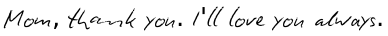
\includegraphics{Images/memo6.png}

That was all it said. It was Shion's writing, without a doubt. It was
his letter, which she had long hoped for. But a sense of unease rippled
through Karan's heart. This―

Mom, thank you. I'll love you always.

These were almost like words of farewell. Like a last kiss, a last
embrace, the last words.

\emph{Mom, thank you. I'll love you always.}

\emph{Goodbye.}

The last unwritten line swirled inside her head.

She stood up. She felt faint. The ceiling, the floor, was spinning.

"Karan!"

"Ma'am!"

She heard Yoming and Lili calling her from far away.

\emph{Shion, wait.}

She reached out and yelled.

\emph{Where are you going? What do you plan to do? Don't tell me―Don't
say you're―}

The Correctional Facility.

She couldn't stop shaking. Karan was seized by the horror of what her
actions had brought about.

She had told him about Safu. Shion was intending to help her escape. He
was the kind of boy who would do something like that. It was something
Karan would have known he would do. She should have known more than
anyone else.

Her ego as a mother emerged fully exposed.

\emph{I shouldn't have told him. Out of all people, I should never have
told Shion.}

\emph{\\
}

\emph{No, Shion. You can't go. You can't be the one that dies.}

\emph{\\
}

\emph{Wait, wait.}

She fell to her knees. In front of her was a small mouse. It was holding
the muffin morsel in both paws, and nibbling at it.

\emph{Nezumi―}

Uncertainty weighed heavily upon her chest, and her heart felt like it
was being wrung.

Where are you? Are you by his side? If you are, then please don't leave
him. I'm begging you. Protect him. Protect him.

\emph{Nezumi!}

The air was thick with the stench of blood, refuse, and sweat. The
people had been crowded into a windowless cargo container, squeezed so
much they could barely move, and they were gasping amidst the stench of
blood, refuse, and sweat. He couldn't breathe. It was hot and humid in
this confined space, and there was no light. It was like they were not
even permitted to breathe.

Beside Shion, a man entering his senior years gave a short gasp. After
several sharp breaths, his head lolled forward. Shion could feel the
man's body begin to convulse repeatedly through his own shoulder, which
was pushed up against him. Shion managed to squirm enough to get his
hand free and place it on the man's mouth.

"Nezumi," he said.

"What?"

"This man―he just died."

"I see," Nezumi responded flatly. "Did he have a heart attack or
something?"

"It might be."

"I see. Well, if he was able to go quickly, maybe it was all the more
lucky for him."

Maybe it was luckier to be able to die here, rather than not being able
to die here. Nezumi's words weren't sarcastic or joking. It was probably
the truth.

As Shion withstood the weight of the deceased man, he thought about the
baby―the small baby he had left along with a dog in the shadows of the
rubble. Would the baby survive?

"Inukashi's probably in a rage right about now." A smile spread thinly
across Nezumi's lips.

"Huh?"

"He'd be flying off the handle because you dumped that baby into his
care. I can just imagine him holding that wailing baby in his arms and
cursing you to high heaven."

"He'd take care of the baby somehow, wouldn't he?"

"Who knows? It's probably already taking everything he's got to take
care of himself and his dogs. Though he probably won't go as far as to
feed the baby to them."

"Inukashi's kind," Shion said firmly. "He wouldn't abandon a helpless
baby."

"Wouldn't he, now?"

"He wouldn't, because he's been raised by a compassionate mother."

"I see. So you're taking advantage of his compassion and kindness to
dump that baby on him, huh?"

"Oh―well, I guess if you put it that way, I have. I didn't realize."

"It might be hard to imagine for Little Mr. Naive, but it's tough.
Babies and puppies are different. Humans take ten times more hassle.
Poor Inukashi, he has to cut back on his own food income to care for
someone else's baby."

"I'll apologize," Shion said simply.

"What?"

"I'll apologize next time I see him."

If you ever do, Nezumi muttered as he shrugged his shoulders.

"But how could you tell?" Shion asked. "How did you know I was thinking
about the baby?"

"We've been together long enough to get sick of each other. I can tell
most of the time. You're pretty easy to read, and―no―" Nezumi cut off
abruptly, and touched his neck. That's not it, he muttered. "I can't
read you at all."

Suddenly, they heard muffled sobbing from somewhere. It was a feeble
voice, belonging to a woman.

"Oh... oh... oh..."

As if dragged along by her weeping, there came an eruption of sobbing
from all over. Some belonged to women, others to men. No one was strong
enough to raise their voice in an anguished cry. Seized by despair,
exhaustion, and fear, they could only weep softly, in a voice that was
barely audible.

As he squatted on the floor hugging his knees, Shion felt the tearful
sniffling of the people soaking into his body.

\emph{Oh, oh, oh...}

\emph{Oh, oh, oh...}

He wanted to cover his ears, but he knew he could not. Even if he did,
it would come seeping in through his skin. It would seep in through his
nostrils, the tips of his hair.

\emph{Oh, oh, oh...}

\emph{Oh, oh, oh...}

Nezumi lifted his chin, and shifted his body slightly.

A song rang out. It was a song Shion had never heard before.

\emph{On the mountaintop far away, the snows are melting}

\emph{Becoming the stream that colours green in the beech wood}

\emph{The fields are now brimming with blossoms}

\emph{And a maiden more beautiful than they}

\emph{Makes a vow of love in the beech wood}

\emph{O youth}

\emph{Wet your feet in the green waters}

\emph{And gallop to me like a deer}

\emph{Before the blossoms fall, come and kiss the maiden's hair}

It was a strange voice. Inukashi had once said that his song was like
the wind, and that it stole the soul away like a wind scattering flower
petals. He was right―Shion could feel his heart being enveloped by the
song, and his soul being beckoned away. In this hopeless space without a
ray of light, for just an instant, flowers bloomed, water babbled, and
the lovers glowed.

The sobbing ceased. The people were enchanted by the song.

Here, in this hellish place, they had heard a beautiful song. It was
like they had encountered a miracle. And it meant that these things
could happen. Even if we've been cast down into the pits of hell, it
doesn't mean we've been torn away whole from beautiful things.

Nezumi caught his breath, and gave a dry cough.

"That was a stretch. There's just not enough air in here. My voice won't
last."

"That's more than enough," Shion reassured him. "It's amazing... I don't
know how to describe it... this is my first time hearing you sing."

"Well, the acoustics here aren't the greatest. There's no orchestra, and
no spotlight. On the stage it would look a little better."

"I'd love to hear it."

"Then let me extend you an invitation. Box seats, the best in the house.
You should bring Inukashi and his baby too."

"I will. I bet even a crying baby would quiet down after hearing you
sing."

"Shion, I was kidding," Nezumi said flatly. "Don't take it seriously."

"Eve." Someone raised his voice in the darkness. "Sing for us, Eve.
Don't stop singing."

"Yeah, Eve. Sing for us."

Shion touched Nezumi's shoulder.

"Everyone wants to hear your song."

"I'm being put through slave labour now, am I?"

"You can save people with your singing. Nezumi, you're amazing." Even
Shion himself knew how inept his words of praise sounded. He was
embarrassed. But he did mean what he said.

\emph{Nezumi, you're amazing.}

"Shion, you can't save people with songs or tales," Nezumi said coldly.
"It'll make them forget their suffering for a little while. But that's
about all it can do. They can't save people in any of the real sense of
the word."

"Eve, sing us 'All the Shimmering Things'," a woman's voice pleaded.

"Geez," Nezumi muttered. "If the Manager finds out I've got fans even in
a place like this, he'd probably burst into tears of joy."

Sing for us, Eve. In this moment, give us your song.

The truck slackened its speed just a little.

"We've passed through the gates," Nezumi muttered, in a voice low enough
that only Shion could hear. Then he began to sing softly again. This
song had a loping tempo, with a touch of melancholy.

\emph{The pearls at the bottom of the sea}

\emph{The stars winking in the night sky}

\emph{And the love that rests in my heart}

\emph{All the shimmering things I surrender to you}

\emph{The sea grows stormy―the pearls disappear}

\emph{The sky grows stormy―the stars disappear}

\emph{But my love will never change}

\emph{Through generations of time}

\emph{Things that shimmer for eternity are just}

The truck stopped. The song cut off abruptly, and atmosphere in the
cargo container froze over again.

"Shion, you hear me?" Nezumi whispered quietly. His voice was heavy now,
completely different from when he was singing. "No matter what happens,
don't get separated from me."

Shion nodded. He clenched his fists.

\emph{No matter what happens, I'll never leave you.}

The truck doors opened.

\emph{"Get off the truck."}

The crowd swarmed off the truck as they were told. Shion followed the
throng. Nezumi nudged him in the ribs.

"That's the Correctional Facility. The place thy breast hath ached
longingly for."

Shion swallowed. He swallowed, and stared at the building before him. It
was a building of white walls. This piece of architecture, almost devoid
of any embellishments and clearly designed to prioritize efficiency, was
something Shion was used to seeing in No. 6.

Apart from the fact that it had very few windows, this building looked
perfectly normal. Its height was about the same as that of the Moondrop,
and four wings about two storeys high protruded from it in different
directions, like arms. The protrusions were perhaps unusual, but not
something that gave off an oppressive or foreboding air.

Shion had expected something more hideous. He had believed it to be
something so hideous, he would not be able to lay his eyes on it.~

The Correctional Facility, which was coloured crimson in the rays of the
setting sun, could easily pass as a medical building. It appeared a
sterile and functional place to the eye.

It was far from what he had imagined.

This was the Correctional Facility―and this was where Safu was.

"This would be the back of the building," Nezumi said. "The front
doesn't look much different, though. So, how is it? Looks a lot more
decent than you imagined, doesn't it?"

"A lot more decent," Shion agreed. "It almost looks like a normal
building."

"Yup. But maybe 'normal' is the scariest thing about it."

\emph{"Walk forward."}

The mob lurched forward. The line fell slightly out of array few metres
ahead of Shion. Someone had collapsed. A soldier approached, and dragged
the person away from the line. It was an old woman wrapped in a tattered
shawl. She was thrown out onto the ground like a rag doll.

"Nezumi, what's gonna happen to her?"

"Don't worry yourself with other people's problems. Even if you knew
what would happen, it's not like you'd be able to do anything."

Another person fell. It was a young woman. Her clothes were torn, and
she buckled to her knees, with her arms covering her bare breasts. One
of the soldiers out of the evenly-spaced line dragged her out promptly.
The same thing was occurring both behind and in front of Shion.

\emph{Are they sorting us?}

Saliva welled up inside his mouth.

\emph{They put us in a confined space, so crowded we couldn't breathe;
put us through confusion, despair, terror... but even after that brutal
experience, now they're selecting those who can still manage to walk in
a straight line?}

"Yeah," Nezumi nodded. "They're sorting us. They're disposing of the
ones who've gotten weak or died during the transport."

"What's the sorting for?"

"I don't know. I still don't know what they're planning to use us for."

"Funny you wouldn't know, huh, even though you seem to know everything
I'm thinking about."

"\emph{Heavens}," Nezumi exclaimed in mock surprise. "To think you can
still be sarcastic in these conditions! That's quite something. Worthy
of praise, my boy."

"I was trained by you―I've toughened up."

"But the real sorting is only starting."

"Just starting, huh..."

They trudged in the blustering wind. In that time, several people
collapsed, and were removed from the line.

Among them were those who lay still, those who shook in the cold, and
those groaning in pain. Without exception, they were all dragged out and
herded into one spot.

\emph{What's going to happen to them? What's going to happen, what's
going to happen? I don't know. Even if I did, there would be nothing I
could do to help it.}

His emotions began to grow numb, starting from the extremities. He was
getting used to atrocity. He was becoming unperceptive to brutal murder.
His thoughts slowed and became sluggish. The death of others no longer
fazed him.

Shion reached out and grabbed Nezumi's arm. He made sure he could feel
the body of flesh at his fingertips.

\emph{Nezumi, keep me as the human I am.}

"There's a chance―" Nezumi dropped his gaze. "―that you might change."

"Huh?"

"Here―in this Correctional Facility, you might change."

"What're you talking about?"

"Maybe the time will come when I'll finally realize―I never knew a thing
about you."

"Nezumi, what are you saying?"

Nezumi clamped his mouth shut, and fell silent.

The people were ordered to stop in front of a set of black doors.

\emph{"Begin entering, starting with the ones at the front. Do not make
any noise."}

The line was divided into three groups, and the first group disappeared
beyond the other side of the door. There was not a sound. A few minutes
later, the door opened again.

"Next."

It was Shion and his group's turn.

\emph{We're going in there?}

Into the interior of the Correctional Facility.

He had steeled himself. He had already made the decision. But he could
not help shrinking back a little. His heart was expanding so much, he
felt like it would burst through his pectoral muscles.

"This was the only way," Nezumi said softly, his gaze staring steadily
ahead. "This was the only way we had, Shion."

"Nezumi..."

"Let's go."

"Yeah."

A gust of wind blew past them. The doors swung open on each side.

"Eve," someone yelled suddenly from somewhere behind. "A song for us. A
song―"

A soldier wordlessly fired his gun. There was the heavy thud of a body
crumpling on the ground. The voice was cut off mid-scream, and the roar
of the wind grew stronger.

Damnit.

Nezumi's lips moved to form the words.

\emph{Damnit. Someday, someday surely I'll―}

\emph{"Move forward."}

Beyond the door was a world of darkness.

It was too dark to decipher how large the space was. Like the cargo
container, they were squeezed in well past the capacity of people it
could hold.

The doors closed.

\emph{Lurch.} The whole room began to shake. And it began to move. They
were moving down at a considerable speed.

"An elevator, huh." The floorplan of the Correctional Facility emerged
in Shion's mind. The blank space underground. This is it. W\emph{e're
moving down into that place.}

They were descending. Descending. It was like they were falling into the
abyss.

Nezumi's arm slid around his waist.

"Hold onto me. No matter what happens, never let go."

"Nezumi, what―"

"We're going to hell together."

The arm around his waist grew tighter.

"But we're coming back alive. Don't forget that, Shion."

"Of course."

The elevator stopped. The darkness wavered.

"We're gonna fall."

Nezumi's voice echoed into a world cloaked in darkness.

\protect\hypertarget{index_split_128.html}{}{}

\hypertarget{index_split_128.htmlux5cux23calibre_pb_132}{%
\subsection{Volume 4}\label{index_split_128.htmlux5cux23calibre_pb_132}}

Volume 4 (tankobon) - Of life and death

It may be a sheepish, foolish, and embarrassing thing to write only
about your most personal thoughts in a space like the afterword.
Thinking back, I realize I've repeated this blunder over and over again,
and even I get sick of it sometimes. So I think I will make this my
last. Will you put up with my complaints one last time? I'm sorry.

This year, I lost two people whom I was very close to. One was Mr. O'oka
Hideaki, a critic and fellow member of our coterie magazine; the other
was Mr. Yamakage Yoshikatsu, of Kodansha's Children's Books Department.
Both supported me as a writer from their respective positions in their
own ways. Being the crude individual that I am, I only realized after I
lost these two how much their support had meant to me, and in my loss,
confusion, and loneliness, I sobbed like a wandering child at sunset.

Mr. Yamakage particularly was my irreplaceable partner in creating the
story of No. 6. He was someone who had stayed with me since Volume 1. He
was also the one who gave this story its title, No. 6. And more than
anything, he has taught me what it means to live on, and what it means
to die.

The following are words that I can't forget.

It was either the beginning of summer, or the end―a time when the
seasons were changing. Mr. Yamakage and I were talking about
this-and-that of my next work inside a taxi, when he said:

"Ms. Asano, you know, these days I've been sweating."

Mr. Yamakage said this suddenly, lowering his voice a little. The
utterance had a hint of a smile in it, like he often used to speak. So?
I thought. Sweat? Isn't it a normal thing to sweat when it gets hot? I
must have had a bemused expression on my face from not understanding the
meaning behind his utterance. But he continued.

"When it's hot, I sweat like I should. It makes me think, wow, I'm
alive."

I realized that it had only been a short time since Mr. Yamakage had
returned to the workplace after recovering from his serious illness; I
nodded then, thoroughly convinced. And now, I contemplate those words
and feel the weight of them all the more.

―Because that is what being alive means. It's sweating when you're hot;
it's crying when you're sad; it's laughing when you're happy. It's
walking straight down a road, and climbing the stairs. It's the days
that pass by, ordinary, mundane, that prove that we are still alive. Mr.
Yamakage taught me that. No. 6 is a story of the boys. It is also a
story of life and death. To a writer like yours truly, who had been
trying to write about life and death as the crux of the story, yet at
the same time in a light and comedic way, perhaps Mr. Yamakage had
stepped beyond his bounds as an editor to convey this message to me.

Ms. Asano, please, truly love that you are alive; cherish it, and
preciously, preciously write about it. Let's make No. 6 that kind of
story―where real human 'life' resides.

He was a brilliant man. He was not afraid at all to live his life
through, and fall into the clutches of death. I wish he could have run
this course with me for a little while―no, for the whole time.

Mr. Yamakage, you went too soon. It's not fair that you just disappeared
like that, engraving yourself in my memories. When I meet you in the
afterworld, I'll be sure to bombard you with complaints. And you'll
probably flash that smile, nod quietly, and apologize in that sheepish
way.

Thank you to everyone who has waited for Volume 4. And I apologize (for
publishing it much, much later than I had originally promised).

And when I was ready to fall to my knees, blurting that maybe this story
was finished too because Mr. Yamakage was gone, I thank everyone who
supported me: Mr. Abe Kaoru, and Mr. Yamamuro Hideyuki, who supported me
in his place; Mr. Kageyama Toru and Mr. Kitamura Takashi, who finished
their jobs like true professionals, and sent me vigorous encouragement
that needed no words. I thank you very, very much.

August 2005

Asano Atsuko

Volume 4 (bunko)

It's an embarrassing story, but when I write afterwords, these days all
I seem to end up with are complaints or excuses. I think it is
absolutely necessary that every story―No. 6 as no exception―should
refuse any complaints or excuses.

For this reason, this time around I've decided to write not any sort of
afterword, but just my thoughts as they come to me.

While I was writing No. 6 Volume 4―or, rather, throughout this whole
series―I've been thinking about what "hope" is.

Hope is believing in the future.

In this world right now, did I really hold a firm belief in the future
as I was writing? I'm still thinking about it (since this series is
still going, after all).

I think and I think, but no matter how much I do, I can't seem to grasp
the answer.

It's not that I've lost hope. In this day and age, I do naturally feel a
sense of imminent danger, to an extent (though it may not be directed
accurately at the right things). But I'm not despairing, nor have I
given up. But if someone were to ask me how much true hope I've got in
my hands―then, well, I've got no choice but to tilt my head in
perplexity. It's certainly an uneasy story...

Hunger, warfare, destruction, poverty, murder, despair...

Change is occurring both on the surface and within people, and these
changes twist and turn; and in our every day lives, like people riding
on a flimsy boat of bamboo leaves in a swift current, we don't know when
we'll be sucked into the whirlpool.

The small light of hope that winked inside me while I was still writing
Volume 1 has now become hard even to make out with my degree of vision.

Has my eyesight gotten worse?

Or has the light gotten weaker?

Hmm? This is starting to sound a lot like a complaint. Note to self:
mind that it doesn't.

Stories detest and avoid complaints and excuses like nothing else. At
the same time, they encourage your struggle to believe in the future.

Stories will not develop or be born from anyone who says, "Well, that's
just how it is" with a skewed and pessimistic outlook; nor does it come
from those who have thrown everything away, saying, "I don't care what
happens anymore". Only those who squint at that tiny ray of light, and
take that hesitant half-step forward―only from that half-step is a story
born.

Perhaps believing in that half-step you take is somehow connected more
largely to believing in the future.

And to you, who has read this story thus far―let's take that hesitant
half-step forward together, why don't we?

Summer 2008

Asano Atsuko
